\section{Performance evaluation}

\subsection{Performance measurement approach}
\label{test-env}
There are two different common approaches to evaluate performance: profiling and benchmarking.

Profiling is used to measure the performance of a given application by adding time measuring and logging code. After the execution has been completed, one can retrace and check how much time had been spent in which function call. This is useful for application developers to find potential bottlenecks and inefficient implemented functions.

Benchmarking addresses mainly the levels underneath the application level, for instance the performance
of the MPI-implementation, the performance of the network and devices. Most interesting results are latencies and bandwidths and their course for various packet or messages sizes. Benchmarking is done by performing numerous iterations of computation and/or communication and measuring the elapsed time.

We used the latter technique to measure the performance of MPI on our test environments, and a combination of both benchmarking and profiling techniques to measure the performance of the different sorting algorithms.

\subsection{Test Environment}
In this section we briefly discuss the architecture of our test environments. 

\paragraph{Pianosa}
\textit{Pianosa} is an old cluster of 30 nodes located at the Department of Computer Science, University of Pisa. Nodes are Intel Pentium III 800 Mhz with a L1 cache of 512KB. The primary memory is of size 1 GB. The operative system is an old distribution of Linux, the Fedora Core 1. On average, the available space on disk in each machine is roughly 15 GB; this capacity obviously limits our tests to data sets of relatively small size. The interconnection network between nodes is a Fast Ethernet, so the MPI support is built on top of the stack TCP/IP. The main weakness of the whole architecture is that the interconnection network is based on a hub: the conflicts at network level becomes not negligible, specially for messages of significant size. This is not just an hypothesis, but something concrete which has been experienced by the group of Parallel Architectures when attempting to define a cost model of MPI. Anyway, even if the architecture has a lot of limitations that can \textit{significantly} affect the performance, Pianosa is a good starting point for testing our algorithms (even from a functional point of view) and to conjecture which architectural characteristics could impair the performance of a Parallel Sorting Algorithm.

\paragraph{PCM}
\label{PCM}
The second target architecture is a cluster of Intel Xeon X5670 (2,93 Ghz) machines located at the Department of Physics, University of Pisa. Each node has 12 cores split in 2 chips (6 cores/chip) and each core allows the execution of two simultaneous threads. Each core has both a L1 cache of 64KB (32 KB dedicated to instructions, 32KB to datas) and L2 cache of 256KB. Each chip has also a L3 cache of 12MB, thus shared by 6 cores. The primary memory is of size 48GB. The disk subsystem is 1x1000 GB SATA II, 7200 RPM, surely faster than the one of Pianosa. The operative system is SUSE Linux Enterprise Server 11. Nodes are interconnected by means of Infiniband. We will use \textit{mvapich2}, a special version of \textit{mpich2} that supports Infiniband. It is clear that the comparison between the old Pianosa and this cluster is unfair: the newer powerful hardware of this architecture will play a key role for the performance of our Sorting Algorithms, both from a quantitative (absolute time completion) and qualitative (scalability) point of view. We will detail all these aspects in the following sections.

\subsection{Cost Model of MPI on the Test Environment}
\label{MPI-cost-model}
\paragraph{The cost of sending a message: the T$\_$send model}
We are interested in evaluating the cost of communications in the test environments because it can help us in understanding the performance behavior of the Sorting Algorithms. Indeed, depending on both the specific architecture and the algorithm, communications may significantly impact the completion time (and so even the scalability) of the algorithm itself. In a simplified view, the cost of sending a message between two tasks located on different processors can be represented by two parameters: the message startup time $T_{setup}$, which is the time required to initiate the communication, and the transmission time $T_{trasm}$ per word, which is mainly determined by the physical bandwidth of the communication channel linking the source and destination processors~\cite{VANN}. In this model, the time required to send a message of size $L$ (that is, for performing a $DAL\_send$ of size $L$) words is then
\[
T_{send}(L) = T_{setup} + L \times T_{trasm}
\]
While accurate for some algorithms and on very simple architectures, this model generally breaks down due to a lot of factors: for instance, the communication pattern of the application, the bandwidth of the interconnection network and, more in general, due to the complexity of the parallel architectures. Despite its weakness, for practical reasons we will refer to the $T\_send$-model to explain the results we achieved.  
The following experimental analysis will try to estimate $T\_send$ on our test architectures by varying the size of the messages and by changing the communication pattern (we will perform the so called ''bisection test'', in which there are two sets of processes, with same cardinality, that exchange messages each other). 

In order to benchmark the performance of the two environments, we decided to use the \textit{Perftest} benchmark suite.

The perftest-package is provided along with the MPI-implementation MPICH, although it can be used in combination with any MPI-implementation. The package contains a few tools to measure the performance of a message passing environment. The two major programs are \textit{mpptest} for measuring point-to-point communication and \textit{goptest} for measuring collective communication. In addition to the classic ping-pong test, mpptest can measure performance with many participating processes (exposing contention and scalability problems) and can adaptively choose the message sizes in order to isolate sudden changes in performance. 

The following test were performed:
\begin{itemize}
	\item Round-trip times between 2 nodes using blocking methods
	\item Blocking bisection times involving from 4 to $n$ nodes
	\item Broadcast times involving from 2 to $n$ nodes
\end{itemize}
In the bisection test the complete system is logically divided into two subsystems and the aggregated bandwidth and latency between the two subsystems is measured. An example of this is splitting the system in two vertically and letting each node in the left half communicate with a node in the right part on a one-to-one basis.

\paragraph{Optimum size of the DAL's communication buffer}
As we said in section~\ref{DAL-impl} we are interested in estimating the \textit{optimum size} for the communication buffer of the DAL layer. In particular, assume that we are performing a $DAL\_send$ of $L$ words. We could send these $L$ words either by performing a single $MPI\_Send$ or, more in general, by performing $X$ $MPI\_Send$. The latter situation is typical in our framework due to the structure of the DAL. Indeed, from section~\ref{DAL-impl}, we remind that each process has its own buffer dedicated to communications; this buffer is of fixed size, let's say $K$ words. Since in general $K < L$, assuming without loss of generality that $L = K \times X$, the cost of sending $L$ words is equal to the cost of performing $X$ $MPI\_Send$ each of size $K$. For each architecture, we have to choose the best value of $K$: indeed, a low value may negatively impact on $T\_send$ (for instance, because of the setup cost of each $MPI\_Send$); a high value could be useless because a too large communication buffer may not give any benefit, rather it may only be a waste of important memory. In order to find the optimal value of $K$, namely the size of the ''static'' communication buffer, we have developed a set of utilities (a program and scripts that share the same prefix  \textit{Tsetup}) that practically estimates the various $T\_send$, $T\_scatter$ and $T\_alltoall$ as functions of $L$ and $X$. 

\paragraph{MPI on Pianosa}
\label{test-env-pianosa}
As stated in the previous paragraph, we focus on determining the \textit{optimum} size of the communication buffer on $Pianosa$. Table~\ref{tsetup-pianosa-n8-M32} shows the time spent by the most used communication primitives (DAL$\_\lbrace$send, scatter, gather, alltoall$\rbrace$) for a message of size 32MB. Each row $i$ of the table is relative to different sizes of the communication buffer. In this way the original message will be sent through $X$ MPI$\_\lbrace$send, scatter, gather, alltoall$\rbrace$ according to the size of the communication buffer ($X \in \lbrace 2^i : i = 0...18 \rbrace$). Table~\ref{tsetup-pianosa-n8-M128} shows another test in which the original message is of size 128MB. In both experiments the parallelism degree is set to 8 (Appendix~\ref{appendixB} shows results with different parallelism degrees). Notice that the parallelism degree is meaningful for scatter, gather and alltoall because it can impact on the overall time spent to carry out the collective communication. By means of these experiments we want to understand which sizes of the communication buffer cause overhead for sending a message with a specific DAL primitive. By looking at the tables we can notice that, from a certain row ahead, some columns are blank (filled with '-'). This means that the overhead of a DAL primitive (column), for a specific size of the communication buffer (row), is become so high that is useless to perform further tests since they would be from one hand meaningless and from the other one a waste of time. Thanks both to these results and to a lot of experiments involving all Sorting Algorithms, we have set the value of the communication buffer to \textbf{32 MB}. 

\begin{table}[h]
\begin{center}
\begin{tabular}{|c|c|c|c|c|c|}\hline
\hline
$\sharp$ MPI calls & MPI size ($\frac{L}{\sharp Sends}$)  & $T\_send$   & $T\_scatter$  & $T\_gather$ & $T\_alltoall$      \\\hline\hline
1 & 32 MB & 3.2885 & 3.2538 & 3.2533 & 4.4369 \\\hline
2 & 16 MB & 3.2846 & 3.2551 & 3.2524 & 5.4570 \\\hline
4 & 8 MB & 3.2847 & 3.2543 & 3.2529 & 5.4825 \\\hline
8 & 4 MB & 3.2851 & 3.2550 & 3.2550 & 5.5014 \\\hline
16 & 2 MB & 3.2862 & 3.2560 & 3.2573 & 5.5177 \\\hline
32 & 1 MB & 3.2867 & 3.2579 & 3.3236 & 19.19259 \\\hline
64 & 512 KB & 3.2918 & 3.2915 & 3.3222 & 25.24587 \\\hline
128 & 256 KB & 3.3006 & 3.2766 & 3.2989 & 27.27086 \\\hline
256 & 128 KB & 3.2847 & 3.2535 & 3.2972 & 40.39969 \\\hline
512 & 64 KB & 3.2848 & 3.2536 & 3.3068 & 69.68816 \\\hline
1024 & 32 KB & 3.2887 & 3.2539 & 3.2965 & 116.116458 \\\hline
2048 & 16 KB & 3.2887 & 3.2558 & 3.3272 & 266.266317 \\\hline
4096 & 8 KB & 3.2894 & 3.2580 & 4.3730 & - \\\hline
8192 & 4 KB & 3.2903 & 3.2645 & 14.13722 & - \\\hline
16384 & 2 KB & 3.2890 & 3.2746 & 39.38740 & - \\\hline
32768 & 1 KB & 3.2938 & 3.3331 & 209.208522 & - \\\hline
65536 & 512 B & 3.3155 & 4.4322 & 353.353234 & - \\\hline
131072 & 256 B & 3.3479 & 5.5415 & - & - \\\hline
262144 & 128 & 6.5900 & 15.15130 & - & - \\\hline
\end{tabular}
\caption{DAL$\_\lbrace send, scatter, gather, alltoall \rbrace$ cost for messages of size 32MB. The cost of a primitive is the time expressed in seconds. }
\label{tsetup-pianosa-n8-M32}
\end{center}
\end{table}

\begin{table}[h]
\begin{center}
\begin{tabular}{|c|c|c|c|c|c|}\hline
\hline
$\sharp$ MPI calls & MPI size ($\frac{L}{\sharp Sends}$)  & $T\_send$   & $T\_scatter$  & $T\_gather$ & $T\_alltoall$      \\\hline\hline
1 & 128 MB & 11.11400 & 10.10070 & 10.10043 & 17.17266 \\\hline
2 & 64 MB & 11.11402 & 10.10094 & 10.10051 & 18.18033 \\\hline
4 & 32 MB & 11.11405 & 10.10100 & 10.10071 & 20.19710 \\\hline
8 & 16 MB & 11.11410 & 10.10082 & 10.10079 & 19.19299 \\\hline
16 & 8 MB & 11.11418 & 10.10045 & 10.10081 & 20.20120 \\\hline
32 & 4 MB & 11.11422 & 10.10075 & 10.10153 & 20.20133 \\\hline
64 & 2 MB & 11.11471 & 10.10116 & 10.10247 & 21.20900 \\\hline
128 & 1 MB & 11.11491 & 10.10205 & 11.10832 & 74.73857 \\\hline
256 & 512 KB & 12.11698 & 12.11658 & 11.10849 & 102.101612 \\\hline
512 & 256 KB & 12.12053 & 11.11130 & 11.10812 & 113.112904 \\\hline
1024 & 128 KB & 11.11405 & 10.10025 & 11.10711 & 174.173785 \\\hline
2048 & 64 KB & 11.11410 & 10.10042 & 11.10515 & 286.285505 \\\hline
4096 & 32 KB & 11.11454 & 10.10067 & 11.11336 & 481.481320 \\\hline
8192 & 16 KB & 11.11424 & 10.10119 & 16.16036 & 1060.1060080 \\\hline
16384 & 8 KB & 11.11446 & 10.10249 & 65.64964 & - \\\hline
32768 & 4 KB & 12.11526 & 10.10489 & 174.173768 & - \\\hline
65536 & 2 KB & 12.11582 & 11.11229 & 692.691751 & - \\\hline
131072 & 1 KB & 12.11758 & 13.13273 & 1196.1195668 & - \\\hline
\end{tabular}
\caption{DAL$\_\lbrace send, scatter, gather, alltoall \rbrace$ cost for messages of size 128MB. The cost of a primitive is the time expressed in seconds.}
\label{tsetup-pianosa-n8-M128}
\end{center}
\end{table}

We conclude this paragraph by showing (Figures~\ref{pianosa-mpi-1},~\ref{pianosa-mpi-2},~\ref{pianosa-mpi-3}) the cost of $DAL\_send$ for small messages. We will have to refer to these figures in the following, when we will show the performance analisys of the algorithms.

\begin{figure}[h]
	\centering
  	\subfloat[Messages of length from 0 to 32 bytes (stride 4 bytes).]{\label{tsend_32}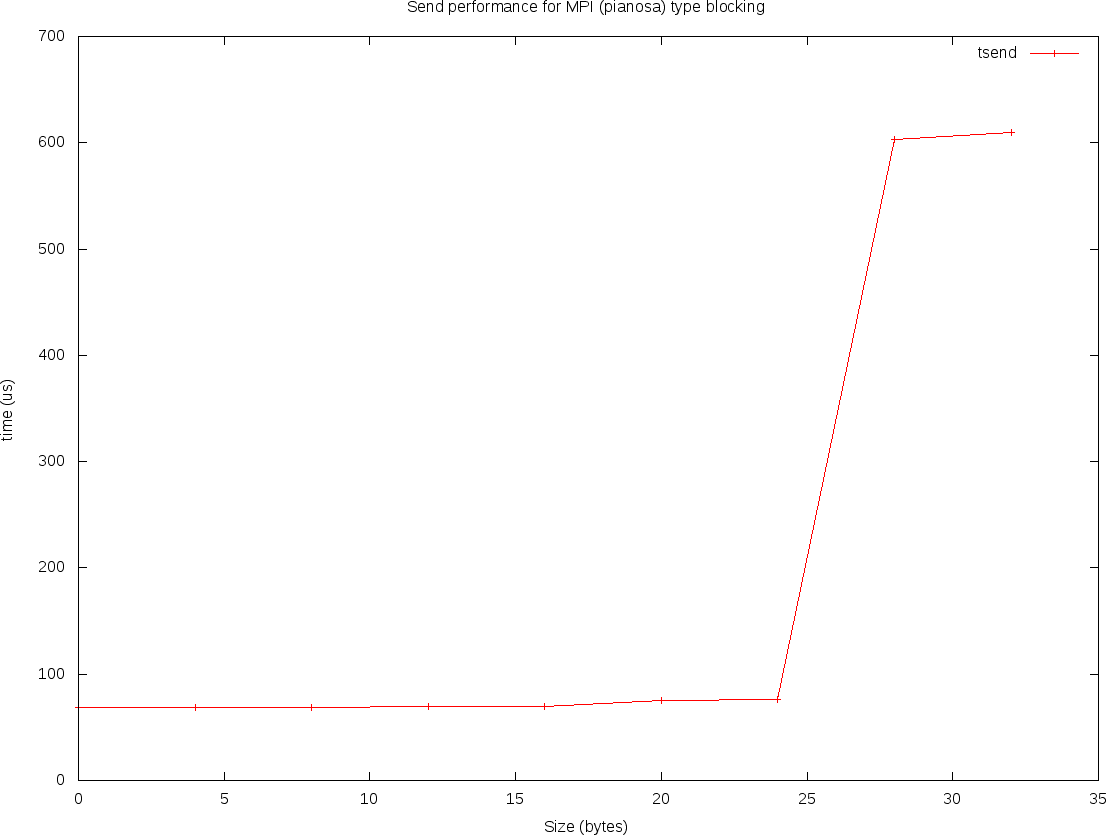
\includegraphics[width=0.4\textwidth]{../tests/mpi_comm_perf/pianosa/tsend_4}}  
	\hspace*{20pt}
  	\subfloat[Messages of length from 0 to 1024 bytes (stride 32 bytes).]{\label{tsend_32}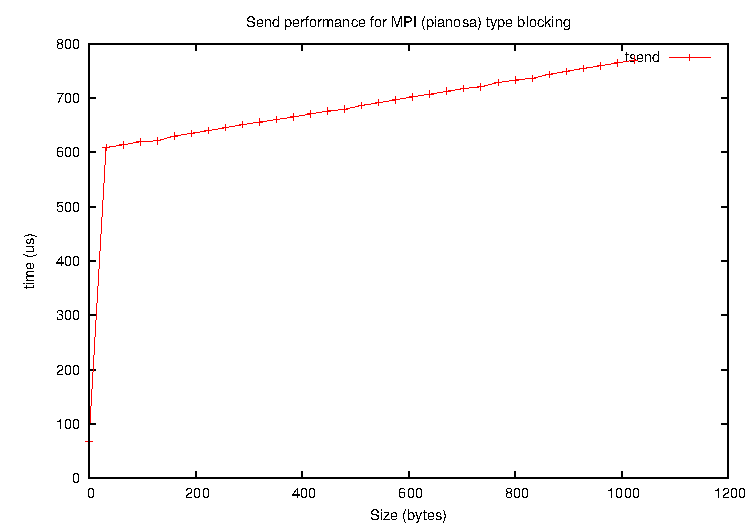
\includegraphics[width=0.4\textwidth]{../tests/mpi_comm_perf/pianosa/tsend_32}}  
	\caption{Performance of blocking send between two processes.}
	\label{pianosa-mpi-1}
	
	\centering
  	\subfloat[Messages of length from 0 to 32768 bytes (stride $2^i$ bytes).]{\label{tsend_logscale}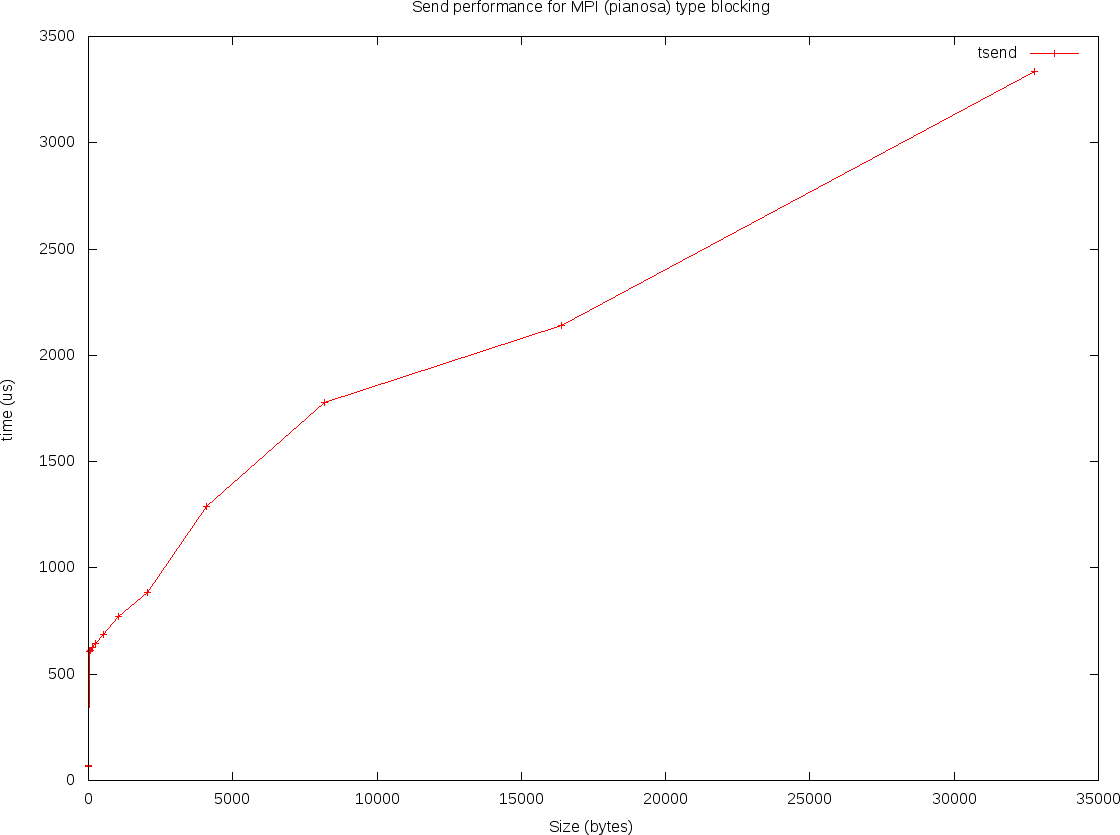
\includegraphics[width=0.4\textwidth]{../tests/mpi_comm_perf/pianosa/tsend_logscale}}  
	\hspace*{20pt}
  	\subfloat[Bisection test with 4, 8 and 16 processors.]{\label{bisect_logscale}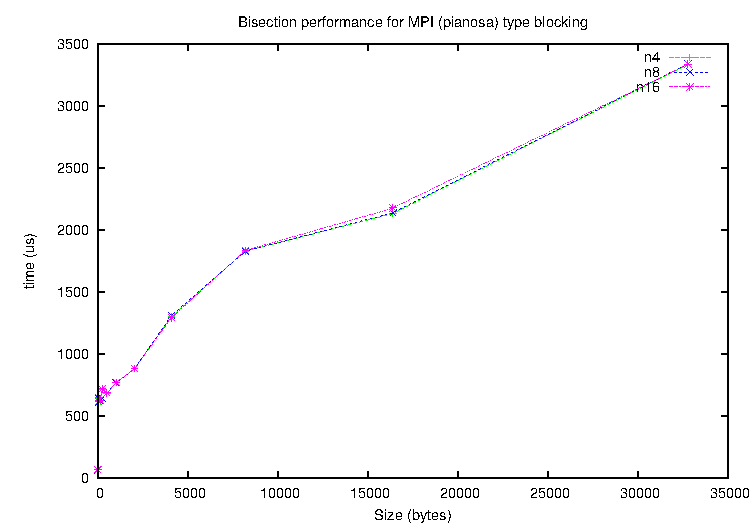
\includegraphics[width=0.4\textwidth]{../tests/mpi_comm_perf/pianosa/bisect_logscale}}  
	\caption{Performance of blocking send and bisection test.}
	\label{pianosa-mpi-2}	
	
	\centering {\label{bcast}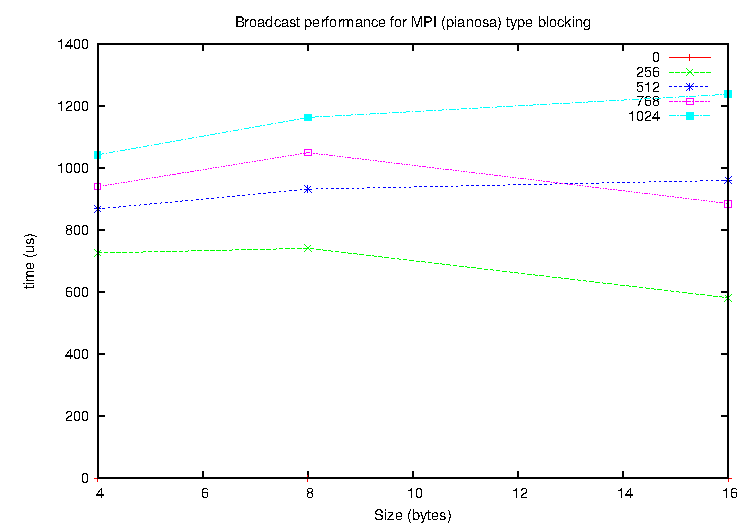
\includegraphics[width=0.4\textwidth]{../tests/mpi_comm_perf/pianosa/bcast}}  
	\caption{Performance of broadcast with 4, 8 and 16 processors.}
	\label{pianosa-mpi-3}
\end{figure}

\clearpage

\paragraph{MPI on IntelXeon X5670}
Same experiments have been executed also on the $IntelXeon\ X5670$ CMP. Tables~\ref{tsetup-xeon-n8-M32} and~\ref{tsetup-xeon-n8-M128} show the time spent by the primitives DAL$\_\lbrace$send, scatter, gather, alltoall$\rbrace$ respectively for messages of size 32MB and 128MB (Appendix~\ref{appendixB} shows results for parallelism degree different from 8). Since the version of MPI that we have used exploits the shared memory to implement (part of) the run-time support of MPI, the latencies of most of MPI primitives is some order magnitude lower that the ones obtained on $Pianosa$.

\begin{table}[h]
\begin{center}
\begin{tabular}{|c|c|c|c|c|c|}\hline
\hline
$\sharp$ MPI calls & MPI size ($\frac{L}{\sharp Sends}$)  & $T\_send$   & $T\_scatter$  & $T\_gather$ & $T\_alltoall$      \\\hline\hline

\end{tabular}
\caption{\textit{IntelXeon X5670.} DAL$\_\lbrace send, scatter, gather, alltoall \rbrace$ cost for messages of size 32MB. The cost of a primitive is the time expressed in seconds. }
\label{tsetup-xeon-n8-M32}
\end{center}
\end{table}

\begin{table}[h]
\begin{center}
\begin{tabular}{|c|c|c|c|c|c|}\hline
\hline
$\sharp$ MPI calls & MPI size ($\frac{L}{\sharp Sends}$)  & $T\_send$   & $T\_scatter$  & $T\_gather$ & $T\_alltoall$      \\\hline\hline

\end{tabular}
\caption{\textit{IntelXeon X5670.} DAL$\_\lbrace send, scatter, gather, alltoall \rbrace$ cost for messages of size 128MB. The cost of a primitive is the time expressed in seconds.}
\label{tsetup-xeon-n8-M128}
\end{center}
\end{table}

\paragraph{MPI on PCM}
$PCM$ is a cluster of $IntelXeon\ X5670$ machines interconnected by means of $Infiniband$. It is interesting to show the cost of the DAL's primitives on this architecture. Tables~\ref{tsetup-pcm-n64-M32} and~\ref{tsetup-pcm-n64-M128} show the time spent by the primitives DAL$\_\lbrace$send, scatter, gather, alltoall$\rbrace$ respectively for messages of size 32MB and 128MB with parallelism degree 64 (Appendix~\ref{appendixB} shows the results for further parallelism degree). Thanks to $Infiniband$, the time elapsed both for exchanging a message and by a collective communication is \textit{at least} two order magnitude lower than the one of $Pianosa$. Moreover, we must notice that the run-time support on $Infiniband$ keeps the cost of a collective communication really close to the one obtained when the run-time support exploits the shared memory, for every parallelism degree; this can be noticed, for instance, by comparing table~\ref{tsetup-pcm-n64-M32} with table~\ref{tsetup-xeon-n8-M32}. In light of what we have shown with these results, the size of the DAL communication buffer can be easily kept to \textbf{32MB}, exactly as on $Pianosa$.

\begin{table}[h]
\begin{center}
\begin{tabular}{|c|c|c|c|c|c|}\hline
\hline
$\sharp$ MPI calls & MPI size ($\frac{L}{\sharp Sends}$)  & $T\_send$   & $T\_scatter$  & $T\_gather$ & $T\_alltoall$      \\\hline\hline

\end{tabular}
\caption{\textit{PCM.} DAL$\_\lbrace send, scatter, gather, alltoall \rbrace$ cost for messages of size 32MB. The cost of a primitive is the time expressed in seconds. }
\label{tsetup-pcm-n64-M32}
\end{center}
\end{table}

\begin{table}[h]
\begin{center}
\begin{tabular}{|c|c|c|c|c|c|}\hline
\hline
$\sharp$ MPI calls & MPI size ($\frac{L}{\sharp Sends}$)  & $T\_send$   & $T\_scatter$  & $T\_gather$ & $T\_alltoall$      \\\hline\hline

\end{tabular}
\caption{\textit{PCM.} DAL$\_\lbrace send, scatter, gather, alltoall \rbrace$ cost for messages of size 128MB. The cost of a primitive is the time expressed in seconds.}
\label{tsetup-pcm-n64-M128}
\end{center}
\end{table}

\begin{figure}[h]
    \centering
    \subfloat[Messages of length from 0 to 32 bytes (stride 4 bytes).]{\label{tsend_1}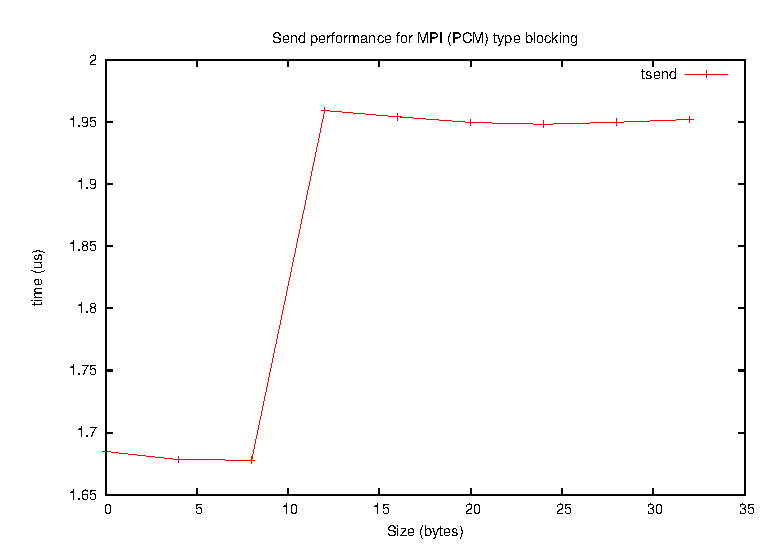
\includegraphics[width=0.4\textwidth]{../tests/mpi_comm_perf/PCM/tsend_1}}  
    \hspace*{20pt}
    \subfloat[Messages of length from 0 to 1024 bytes (stride 32 bytes).]{\label{tsend_2}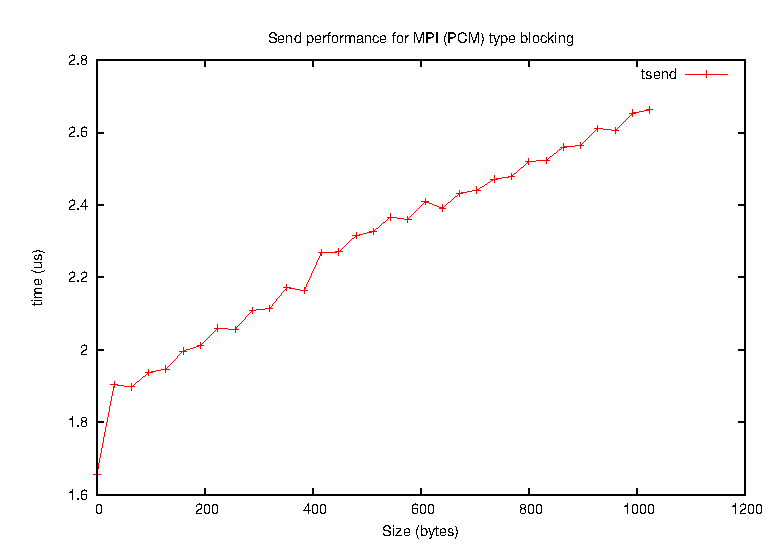
\includegraphics[width=0.4\textwidth]{../tests/mpi_comm_perf/PCM/tsend_2}}  
    \caption{Performance of blocking send between two processes.}
    \label{PCM-mpi-1}
    
    \centering
    \subfloat[Messages of length from 0 to 32768 bytes (stride $2^i$ bytes).]{\label{tsend_logscale}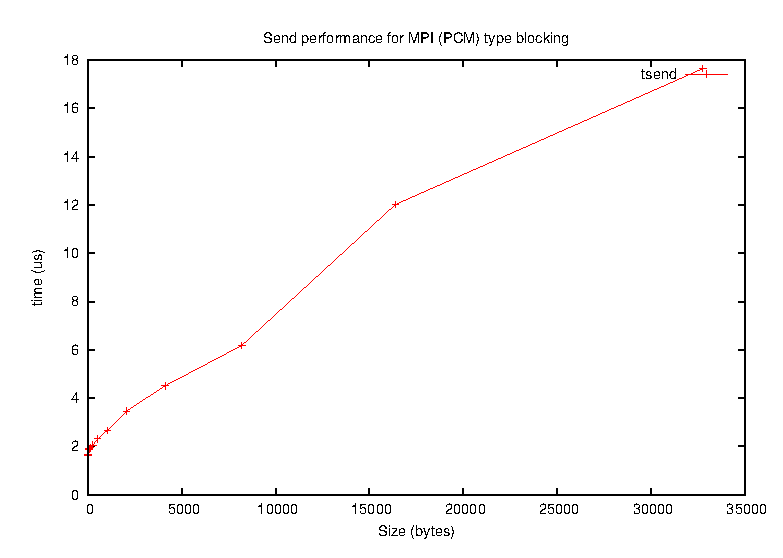
\includegraphics[width=0.4\textwidth]{../tests/mpi_comm_perf/PCM/tsend_logscale}}  
    \hspace*{20pt}
    \subfloat[Bisection test with 4, 8, 16, 32 and 64 processors.]{\label{bisect_logscale}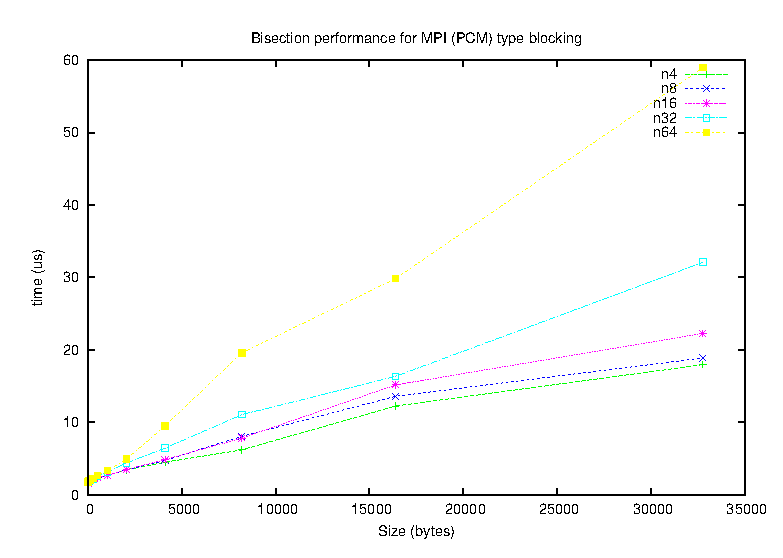
\includegraphics[width=0.4\textwidth]{../tests/mpi_comm_perf/PCM/bisect_logscale}}  
    \caption{Performance of blocking send and bisection test.}
    \label{PCM-mpi-2}   
    
    \centering {\label{bcast}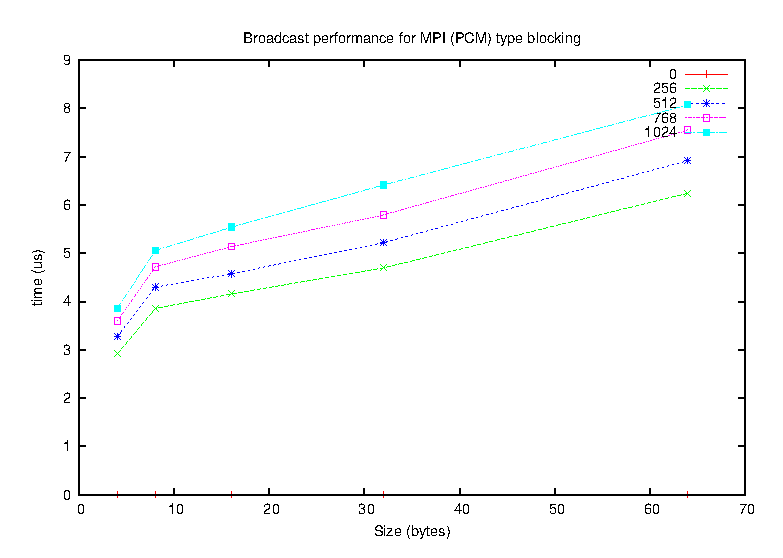
\includegraphics[width=0.4\textwidth]{../tests/mpi_comm_perf/PCM/bcast}}  
    \caption{Performance of broadcast with 4, 8, 16, 32 and 64 processors.}
    \label{PCM-mpi-3}
\end{figure}

\clearpage

\subsection{Algorithms Efficiency}
In this section, we are going to analyze the theoretical Algorithm Efficiency defined in~\ref{terminology}. For the sake of commodity, we report here the definition. Given
\begin{itemize}
\item $N$, the parallelism degree; 
\item $m$, the number of steps of the algorithm;
\item $X_i$, a random variable which counts the number of active processes that contribute to the calculation during the step $i$.
\end{itemize}
We defined the Algorithm Efficiency $\varphi$ as:
\begin{center}
$\varphi = \frac{\sum_{i=0}^m E[X_i]}{N \times m} $
\end{center}
In this section we want to give an idea of how many of the $N$ processes with which a Sorting Algorithm is executed are actually exploited by the parallel logic of the algorithm. In the following we show the Algorithm Efficiency of each Sorting Algorithm.

\begin{itemize}
\item \textbf{Mergesort, Quicksort.} $\varphi = \frac{\sum_{i=0}^{ \lceil \log_2{N} \rceil} 2^i}{N \times \lfloor \log_2{N} + 1 \rfloor} $
\begin{enumerate}
\item $N = 16 \rightarrow \frac{31}{80} \approx 0.39$
\item $N = 32 \rightarrow \frac{63}{192} \approx 0.33$
\end{enumerate}

\item \textbf{K-Way Mergesort.} $\varphi = \frac{\sum_{i=0}^{ \lceil \log_k{N} \rceil} min ( k^i, N )}{N \times \lfloor \log_k{N} + 1 \rfloor } $
\begin{enumerate}
\item $N = 16, k = 4 \rightarrow \frac{21}{48} \approx 0.44$
\item $N = 16, k = 8 \rightarrow \frac{25}{48} \approx 0.52$
\end{enumerate}

\item \textbf{Bitonicsort.} $\varphi = \frac{\sum_{i=0}^{(\log_2{N})^2} N}{N \times (\log_2{N})^2} = 1 $
\item \textbf{Bucketsort, Samplesort.} In these algorithms steps have the characteristic of being heterogenous: a first step is the local sorting of datas, than a step of sampling and finally a step for building buckets. A process will never sleep, so we trivialy have: $\varphi = 1$.

\item \textbf{Load Balanced Mergesort, K-Way Load Balanced Mergesort.} Trivialy, $\varphi = 1$. Indeed, these algorithms have been conceived exactly for maximizing the number of processes which contributes to the sorting during all the computation.

\end{itemize}

\subsection{Performance analysis of the algorithms}
\label{performance-analysys}
We said in~\ref{sort-fram} that sorting a data set is a computation described by a \textit{5-tuple} $\langle n$, $M$, $s$, $\Lambda$, $\sigma \rangle$, with $n$ the parallelism degree, $M$ the size of the data set, $s$ a seed for generating the data set, $\Lambda$ the algorithm and $\sigma$ a set of parameters depending on $\Lambda$. In reality, $\sigma$ is significative just for some algorithms; for instance, it can specify the \textit{stencil} (communication pattern) for the processes of a parallel algorithm or the value of ''\textit{K}'' in algorithms like \textit{K-way mergesort}. For each $\Lambda$, we will run single-shot computations (that is, there are not streams of data sets to sort) by varying $n$, $M$, $s$. Initially, $\sigma$ will be fixed for every computations. It is a convention that we will refer to \textit{small}, \textit{large} or \textit{huge} data sets for sizes that are respectively a few MBs, hundreads of MBs and (at least) GBs. 

In order to analyze the performance of the algorithms from different perspective (e.g.: scalability of the specific algorithm, comparison of the time completion required by different algorithms to sort a specific data set and so on) we are going to show different types of graphics. Each graphic is defined by a 3-tuple $\langle x, y, plot \rangle $, where $x$ is the variable on the X axis, $y$ the variable on the Y axis and $plot$ a parameter that identifies a specific shape of that graphic. In particular, given $T$ the time completion of a computation, we will focus on the following graphics:
\begin{enumerate}
\item fixed $M$, a graphic $\langle n, T, \Lambda \rangle $ is necessary to see which is \textit{the ''best'' algorithm} for sorting a data set of a certain $M$ on a specific architecture. Here, we refer to the ''best'' algorithm(s) as the one(s) that is able either to sort faster a specific data set, to scale better or a combination of them. 
\item fixed $\Lambda$, a graphic $\langle n, T, M \rangle$ is useful to see the \textit{scalability} of $\Lambda$ on a specific architecture. Different shapes shows the scalability of $\Lambda$ for different sizes of the data set.
\item fixed $\Lambda$, a graphic $\langle M, T, n \rangle$ to show (as before) the behaviour of $\Lambda$ on a specific architecture, but from a different perspective. 
\item a graphic $\langle M, T, \Lambda \rangle$ to understand which algorithm \textit{should} be used if the target architecture allowed a parallelism degree of at most $n$. These graphics could be used as ''experimental cost models'', in sense that in principle they could predict the performance of a Sorting Algorithm on such architectures that are ''similar'' to our target architectures. Here, ''similar'' refers mainly to CPUs, memory hierarchies, I/O subsystem, interconnection structure.  
\end{enumerate}

The parameters of the computations will take the following values:
\begin{itemize}
\item $\Lambda \in \lbrace$Sequentialsort, Bitonicsort, Samplesort, Bucketsort, Mergesort, Quicksort, K-Way Mergesort, Load-Balanced Mergesort, Load-Balanced Multi-Way Mergesort$\rbrace$;
\item $n \in \lbrace$1, 2, 4, 8, 16, 32, 64, 128, 256$\rbrace$; notice that the maximum value that $n$ can take depends on the specific architecture. 
\item $M \in \lbrace 2^{10 + i} : i = 0, ..., 25\rbrace$ elements (integers). So $M$ takes values from a few kilobytes to tens of gigabytes (recall that each integers is usually represented through 4 bytes).
\end{itemize} 

For each target architecture, first we will focus on analyzing the scalability of each Sorting Algorithms (graphics 2, 3). Then, we will compare them by fixing the size of the data set and showing which algorithm sorts it faster, for different parallelism degrees (graphic 1). Finally, we will show and explain which is the best algorithm for our target architectures. 

\subsubsection{Pianosa}
On this architecture, due to the lack of space on disks, we will be able to test Sorting Algorithms for data sets of size at most 4GB, namely 1G integers. Further, given the results of tests shown in~\ref{test-env-pianosa}, the size of the communication buffer of the DAL layer has been set to 32MB. We have also practically experienced that a larger buffer, in general, does not give significant benefits, while a shorter one impair a little the Time Completion.

\paragraph{Scalability of Sorting Algorithms}
Figures~\ref{NxTxM} and~\ref{MxTxN} show the Time Completion of Sorting Algorithms on Pianosa.

If the data set is \textbf{small} (i.e. of size up to 64MB) there is not any Sorting Algorithms that shows a good scalability. Even worse, if we look at Figure~\ref{NxTxA-small} we notice that by increasing the parallelism degree we obtain an increase of the Time Completion too. In reality, this behaviour is not surprising. The cost of \textit{Sequentialsort} (that is, the cost of the standard \textit{ANSI qsort}, since the data set surely fits the primary memory) for small data sets varies between a few seconds and tens of milliseconds, that is the same order magnitude of $T\_send( \sim KB )$ (see~\ref{test-env-pianosa} for more details). This means that the cost of communications between processes has a significative impact on the final performance of Sorting Algorithms. From a qualitative point of view, the higher the parallelism degree, the higher both the number of communications and the overall time spent in sending datas, so higher is even the overhead introduced by the parallelization. This is why Sorting Algorithms cannot scale and usually exhibit a Time Completion even worse than the one of \textit{Sequentialsort}.

Things are a little bit different when the data set is \textbf{large}, namely when its size is between 128MB and 512MB. Figure~\ref{NxTxM} clearly shows that there is not any algorithm that scales. Bucketsort and Samplesort have a little improvement passing from $n=2$ to $n=4$, but nothing extraordinary. However, if the data set is of 512MB, the parallelization is useful to lower the Time Completion with respect to the one of \textit{Sequentialsort}. Figure~\ref{sequential-pianosa} shows that, for sorting 512 MB, \textit{Sequentialsort} takes roughly 400s, while all Sorting Algorithms, except Quicksort, are able to lower it up to roughly 200s with just $n=4$. Unfortunately, we do not obtain any further improve neither moving from $n=4$ to $n=8$ nor considering a smaller data size (with just $M=256MB$ the parallelizzation gain is not significative). Reasons are quite obvious. From one hand, if we increase the parallelism degree the negative impact of communications is greater than the gain coming from having more computational units (working on smaller partitions).  From the other hand, $M=512MB$ means a jump to an important computational grain: indeed, moving from $n=2$ to $n=4$ guarantees processes to work with a partition of the data set that is still significative; this explains why some Sorting Algorithms shows a gain in terms of Time Completion within this range of processes. If we further increase $n$ up to $16$, processes have to work on smaller partitions, which let the parallelization in some sense useless.

Summarizing, we have just seen that Sorting Algorithms do not scale with data sets of sizes up to a few hundreads of megabytes. Moreover, for small data sets, \textit{Sequentialsort} even outperforms all other parallel algorithms. Reasons of this behaviour are mainly two: the fine grain computation on a few datas \textit{and} the cost of communications, which becomes predominant on a cluster. Now, we focus on \textbf{huge} data sets. Even if the computation is still of fine grain, now each process works with larger partitions of the data set. Besides, notice that in our tests the increment of the data set size is exponential (doubles at each test). This means that processes spend greatly more time in computation than what happened for large data sets. Just as an example, think to two data sets $A$ and $B$, the former of size $\sharp A = 256$ MB, the latter of size $\sharp B = 2$ GB; both of them have to be sort with the same generic Sorting Algorithm. Assume that the parallelism degree is $n=8$. In the first phases of the algorithm, each process works with partitions of sizes respectively $local_A = \frac{\sharp A}{n} = 32$ MB and $local_B = \frac{\sharp B}{n} = 256$ MB. It is clear that a lot of more time is spent just to sort local partitions. If the Sorting Algorithm has a parallel logic such that both the workload keeps balanced among processes and the amount of communications do not overcome the time spent in computations, then a Sorting Algorithm \textit{can} scale. For instance, assume that the Sorting Algorithm in question is the \textit{Samplesort}. During the various steps of the algorithm, processes work with partitions of similar sizes and, except in both the initial scattering and final gathering phases, on average they send $local_{\lbrace A,B \rbrace}$ datas (see~\ref{Samplesort}). On the other hand, assume that the Sorting Algorithm is the \textit{Mergesort}. It is still true that when the data set is $B$, processes have a larger computation phase: but it is also true that the workload tends to be concentrated on a few processes through $log_2{n}$ phases of costly communications (in the best case, a process sends $local_{\lbrace A,B \rbrace}$, while in the final step of the algorithm a process has to send $\frac{\sharp\lbrace A,B\rbrace}{2}$ datas). Therefore, this example shows intuitively how for some Sorting Algorithms (in our case \textit{Samplesort}) the increase of the data set size implies a larger increment of the computation phase with respect to the communication phase, while for other algorithms (in our case \textit{Mergesort}) the workload gets unbalanced after costly phases of communications. This example was necessary to give an idea of why we obtain the behaviour shown in Figure~\ref{NxTxM}, where for huge data sets only some Sorting Algorithms significatively improve their Time Completion by increasing $n$ (\textit{Bucketsort}, \textit{Samplesort}, \textit{Load-Balanced (Multi-Way) Mergesort}, \textit{Bitonicsort}), while other either do not get better (\textit{Mergesort}, \textit{4-Way Mergesort}) or even worsen (\textit{Quicksort}). However, notice that in every case the scalability is far away from the ideality. 

Finally, we observe an interesting behaviour. We consider again the Time Completion of Sorting Algorithms in case of huge data sets. Figure~\ref{NxTxM} shows that algorithms like \textit{Samplesort} (Figure~\ref{NxTxM-samplesort}) and \textit{Load-Balanced Multi-Way Mergesort} (Figure~\ref{NxTxM-lbkmergesort}) exhibit the best gain when the parallelism degree grows from 2 to 4, while by passing to 8 and even worse to 16 the gain tends to diminish. There are no valid reasons to think that with higher parallelism degree the gain restarts to grow. On the other hand, \textit{Bitonicsort} (Figure~\ref{NxTxM-bitonicsort}) does not obtain a significative gain with parallelism degrees up to 8, while passing from 8 to 16 the gain nearly halves. Therefore, it would be interesting to study the behaviour of \textit{Bitonicsort} for higher parallelism degree; this will be our matter of study on another target architecture.

\begin{figure}[t]
	\begin{center}
		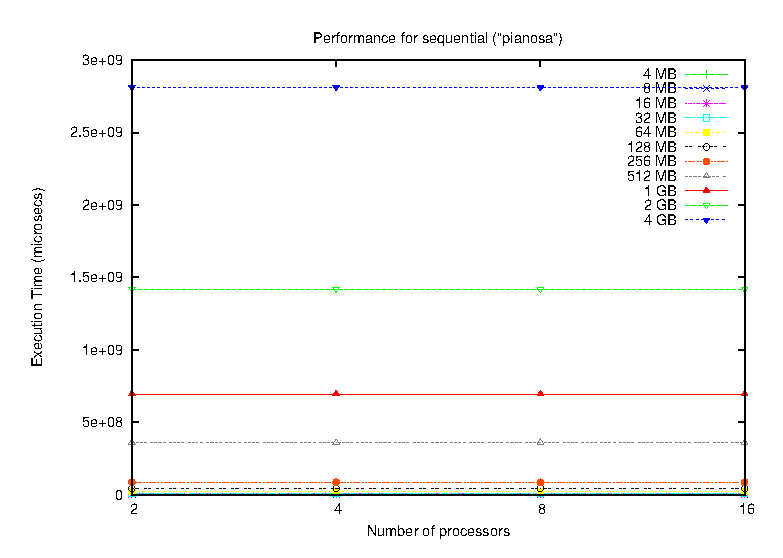
\includegraphics[scale=0.6]{plots/test_01_pianosa/NxTxM/sequential_pianosa_NxTxM}
	\end{center}
  	\caption{\textit{Pianosa}. Completion Time for the Sequentialsort.}
  	\label{sequential-pianosa}
\end{figure}

\begin{figure}[h]
	\centering
	\subfloat[Quicksort.]{\label{NxTxM-sequential}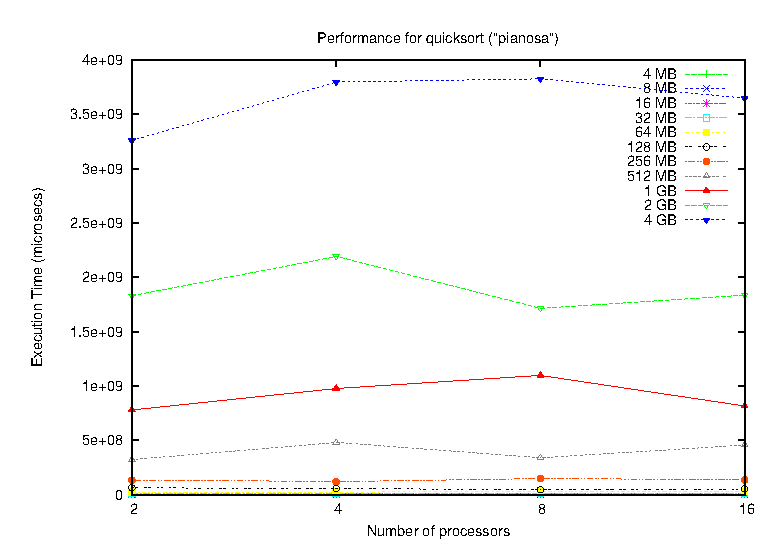
\includegraphics[width=0.4\textwidth]{plots/test_01_pianosa/NxTxM/quicksort_pianosa_NxTxM}} 
	\hspace*{20pt}	
  	\subfloat[Bitonicsort.]{\label{NxTxM-bitonicsort}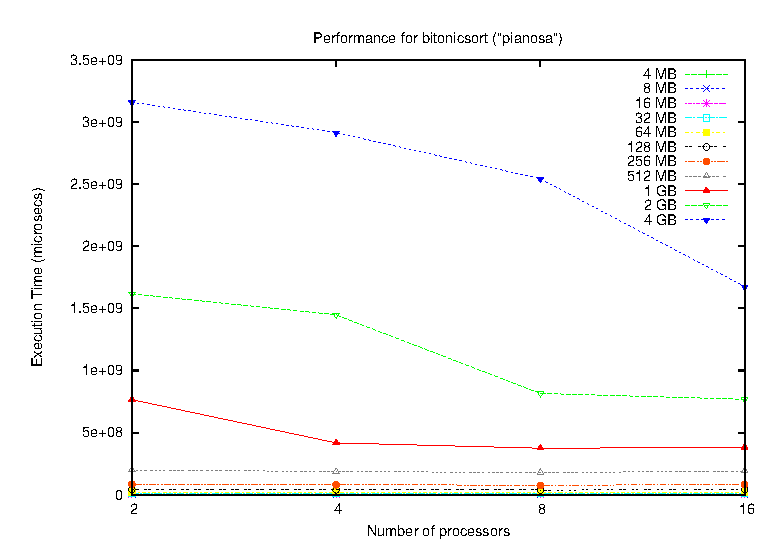
\includegraphics[width=0.4\textwidth]{plots/test_01_pianosa/NxTxM/bitonicsort_pianosa_NxTxM}} 
	
	\centering
	\subfloat[Bucketsort.]{\label{NxTxM-bucketsort}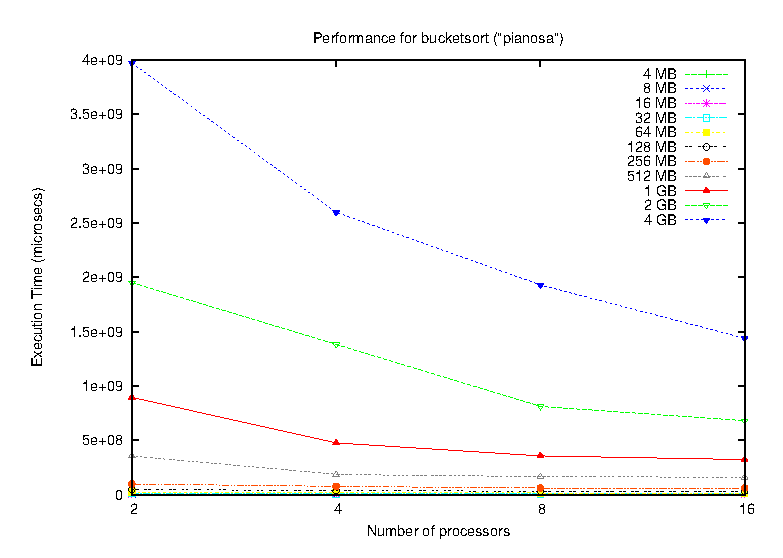
\includegraphics[width=0.4\textwidth]{plots/test_01_pianosa/NxTxM/bucketsort_pianosa_NxTxM}} 
  	\hspace*{20pt}
  	\subfloat[Samplesort.]{\label{NxTxM-samplesort}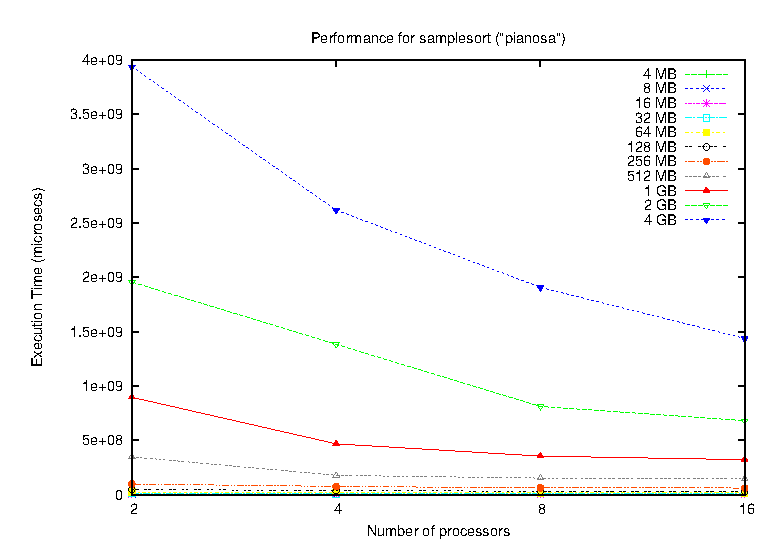
\includegraphics[width=0.4\textwidth]{plots/test_01_pianosa/NxTxM/samplesort_pianosa_NxTxM}} 
	
	\centering
  	\subfloat[Mergesort.]{\label{NxTxM-mergesort}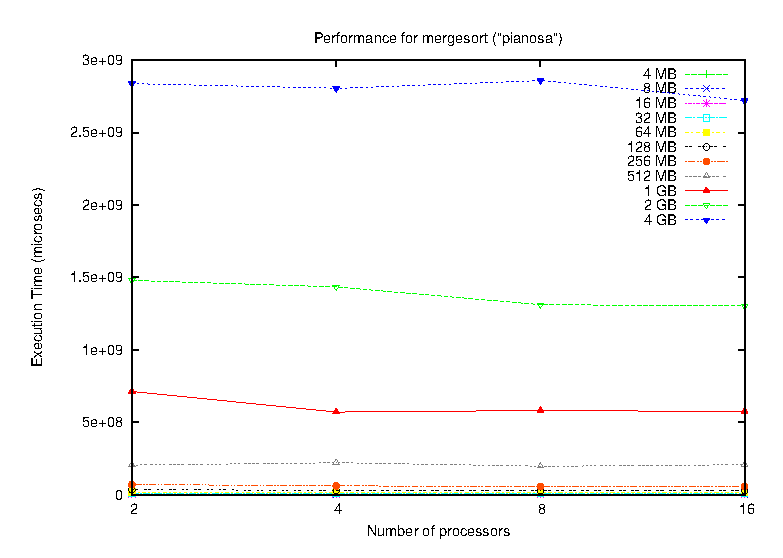
\includegraphics[width=0.4\textwidth]{plots/test_01_pianosa/NxTxM/mergesort_pianosa_NxTxM}}   
  	\hspace*{20pt}  
  	\subfloat[4-Way Mergesort.]{\label{NxTxM-kmerge}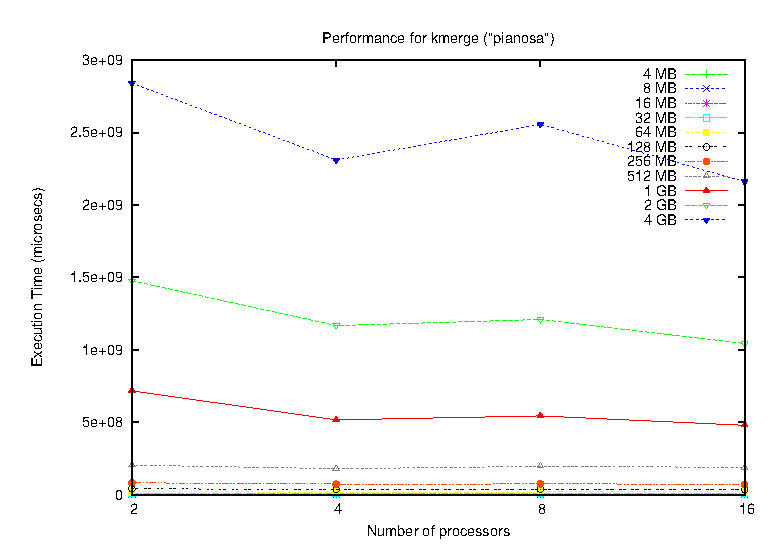
\includegraphics[width=0.4\textwidth]{plots/test_01_pianosa/NxTxM/kmerge_pianosa_NxTxM}} 
	
	\centering
  	\subfloat[Load-Balanced Mergesort.]{\label{NxTxM-lbmergesort}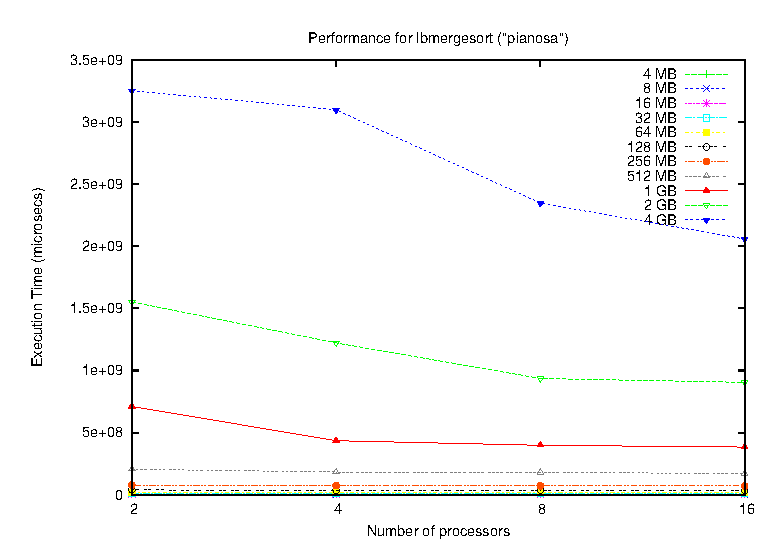
\includegraphics[width=0.4\textwidth]{plots/test_01_pianosa/NxTxM/lbmergesort_pianosa_NxTxM}} 
  	\hspace*{20pt}  
  	\subfloat[Load-Balanced Multi-Way Mergesort.]{\label{NxTxM-lbkmergesort}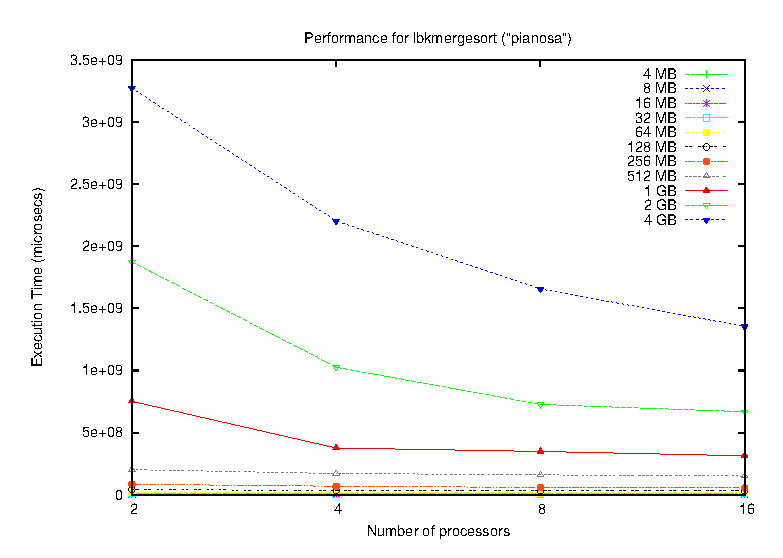
\includegraphics[width=0.4\textwidth]{plots/test_01_pianosa/NxTxM/lbkmergesort_pianosa_NxTxM}} 	
  	
	\caption{\textit{Pianosa}. Time Completion of Sorting Algorithms by varying the parallelism degree. Each shape on a graphic represents the Time Completion of a certain Sorting Algorithm for a data set of specific size.}
	\label{NxTxM}
\end{figure}
 
\begin{figure}[!ht]
	\centering
	\subfloat[Quicksort.]{\label{MxTxN-sequential}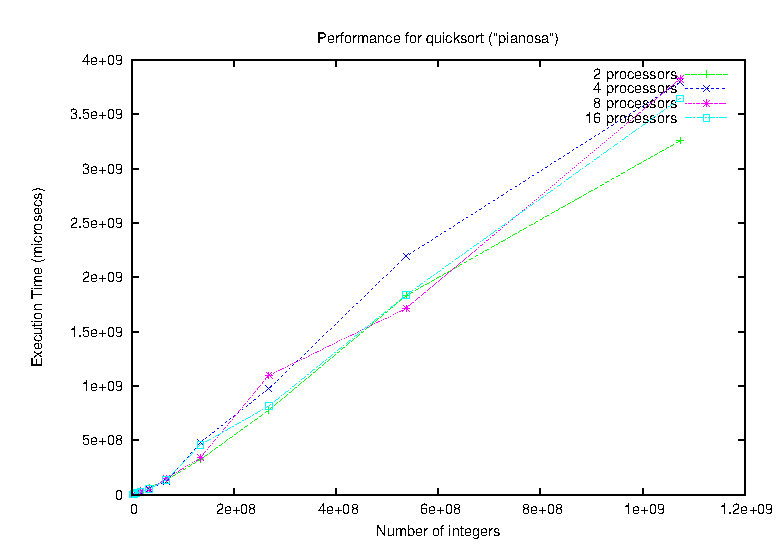
\includegraphics[width=0.4\textwidth]{plots/test_01_pianosa/MxTxN/quicksort_pianosa_MxTxN}} 
	\hspace*{20pt}	
  	\subfloat[Bitonicsort.]{\label{MxTxN-bitonicsort}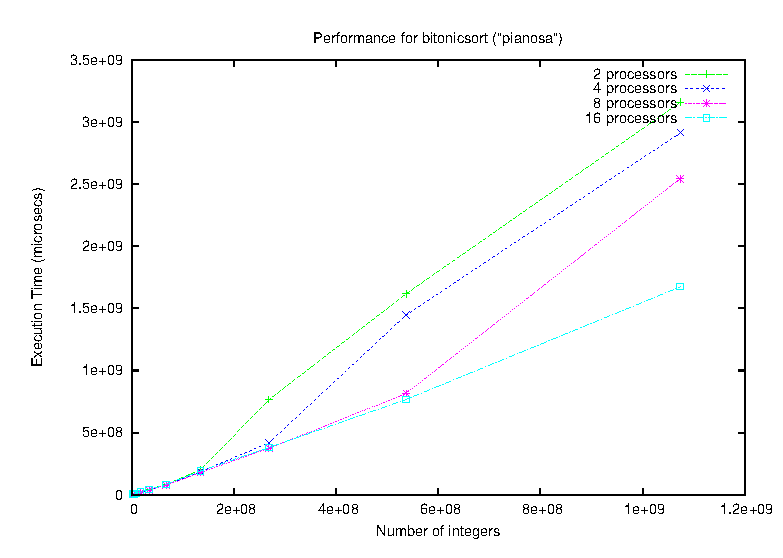
\includegraphics[width=0.4\textwidth]{plots/test_01_pianosa/MxTxN/bitonicsort_pianosa_MxTxN}} 
  		
	\centering
	\subfloat[Bucketsort.]{\label{MxTxN-bucketsort}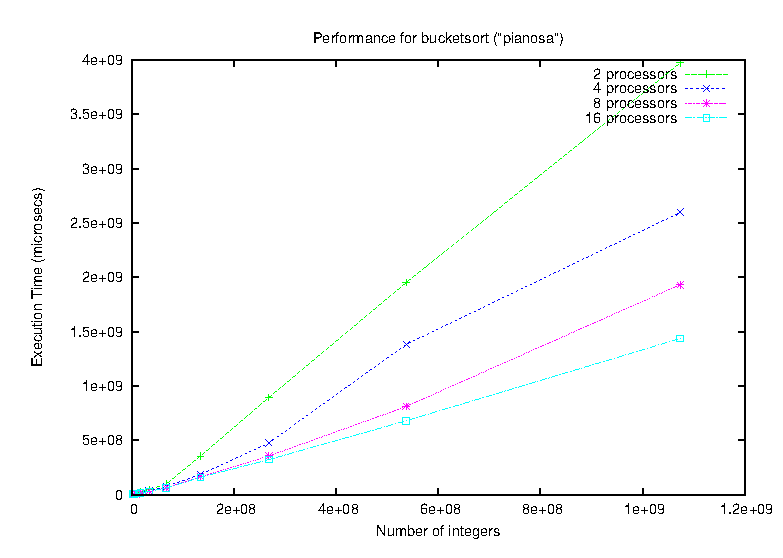
\includegraphics[width=0.4\textwidth]{plots/test_01_pianosa/MxTxN/bucketsort_pianosa_MxTxN}} 
  	\hspace*{20pt}
  	\subfloat[Samplesort.]{\label{MxTxN-samplesort}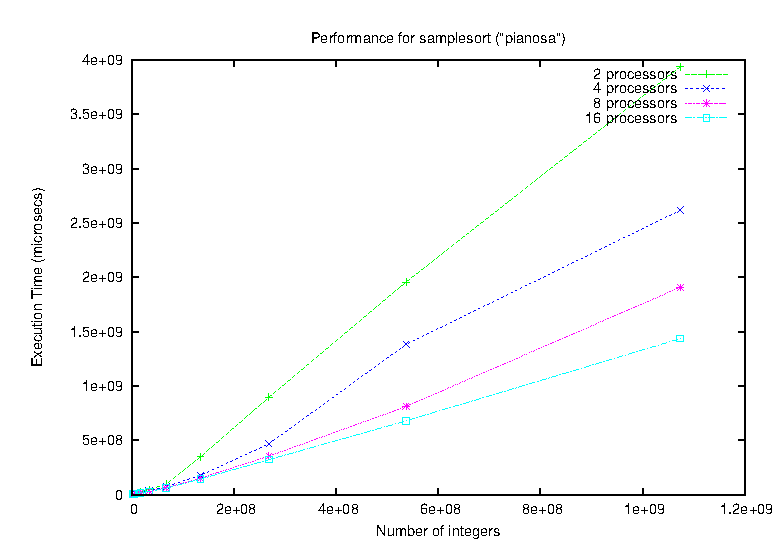
\includegraphics[width=0.4\textwidth]{plots/test_01_pianosa/MxTxN/samplesort_pianosa_MxTxN}} 
	
	\centering
  	\subfloat[Mergesort.]{\label{MxTxN-mergesort}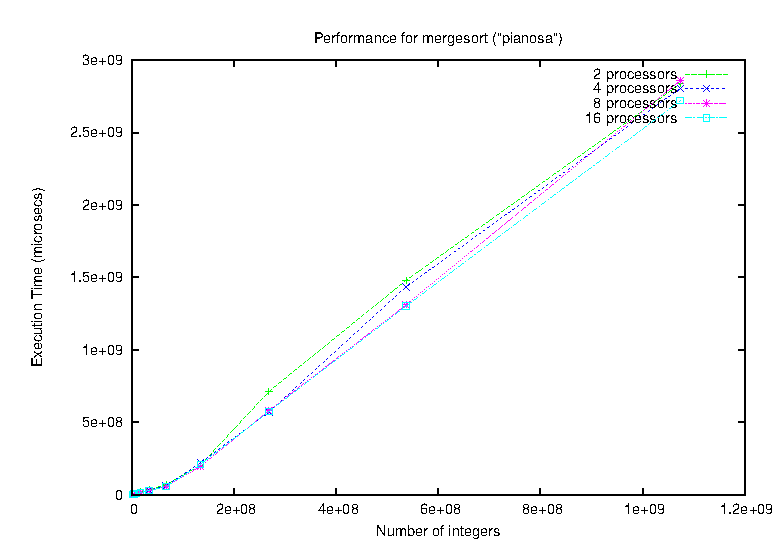
\includegraphics[width=0.4\textwidth]{plots/test_01_pianosa/MxTxN/mergesort_pianosa_MxTxN}}   
  	\hspace*{20pt}  
  	\subfloat[4-Way Mergesort.]{\label{MxTxN-kmerge}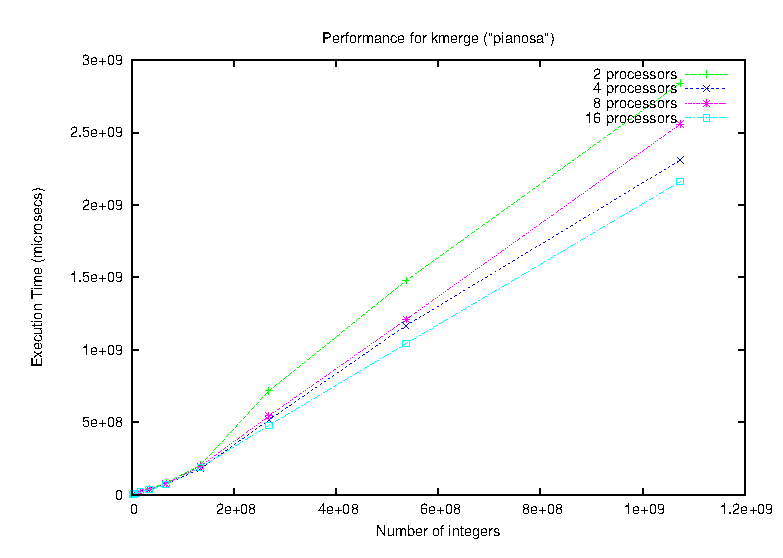
\includegraphics[width=0.4\textwidth]{plots/test_01_pianosa/MxTxN/kmerge_pianosa_MxTxN}} 
	
	\centering
  	\subfloat[Load-Balanced Mergesort.]{\label{MxTxN-lbmergesort}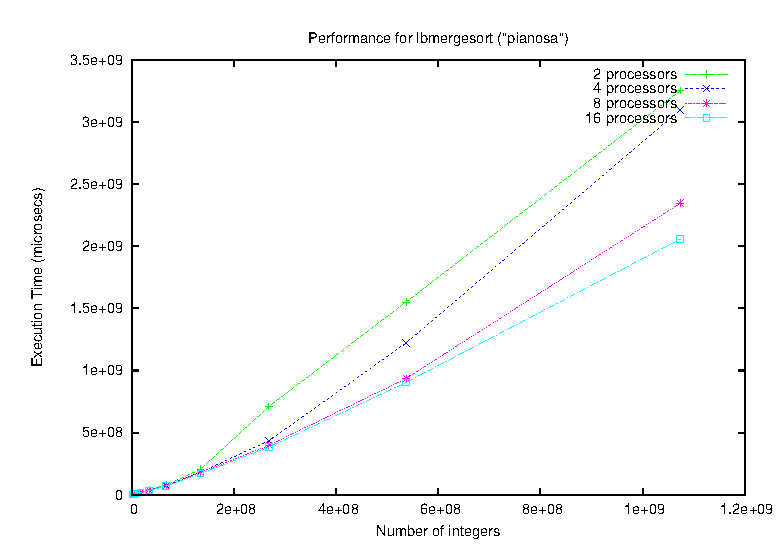
\includegraphics[width=0.4\textwidth]{plots/test_01_pianosa/MxTxN/lbmergesort_pianosa_MxTxN}} 
  	\hspace*{20pt}  
  	\subfloat[Load-Balanced Multi-Way Mergesort.]{\label{MxTxN-lbkmergesort}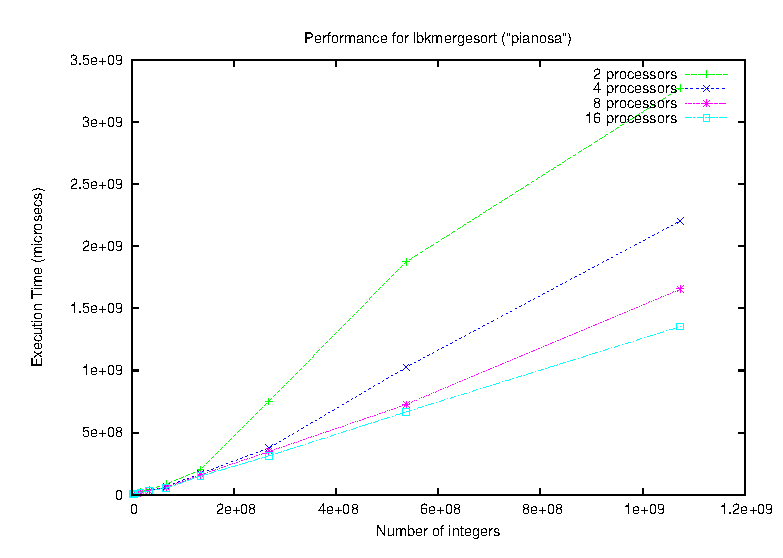
\includegraphics[width=0.4\textwidth]{plots/test_01_pianosa/MxTxN/lbkmergesort_pianosa_MxTxN}} 
  	
	\caption{\textit{Pianosa}. Time Completion of Sorting Algorithms for increasing sizes of the data set. }
	\label{MxTxN}
\end{figure} 
  
\paragraph{Comparison between Sorting Algorithms}
In the previous section we have analyzed the scalability of singles Sorting Algorithms for different sizes of the data set. Now, we focus on determining the best Sorting Algorithm, in terms of Time Completion, for different sizes of the data set. First of all, recall that whether a data set fits the primary memory, a call to \textit{Sequentialsort} is simply a call to the standard \textit{ANSI qsort} (see chapter~\ref{sort-fram}). Therefore, in case of \textbf{small} data sets, the \textit{Sequentialsort} is the best algorithm we can use. Indeed, as we have already anticipated, in these cases the overhead of the parallelization is greater than the time that we would spend in a sequential, optimized computation, like the one of \textit{qsort}. On the other hand, things are obvioulsy different for larger data sets. Figures~\ref{NxTxA-large} and~\ref{NxTxA-huge} can be used to derive which algorithms exhibit the best Time Completions respectively for large and huge data sets. First, we consider the case of \textbf{large} data sets. 
Aside the \textit{Quicksort}, which suffers the unbalancing of the load among processes (see Appendix~\ref{appendix} for more details), most of the Sorting Algorithms outperform \textit{Sequentialsort}, at least when the size of the data set is greater than 4M integers. At least up to parallelism degree 16, the best algorithm is \textit{Mergesort}: in the best case, it is able to lower the Time Completion of \textit{qsort} of roughly 25$\%$ (see Figure~\ref{NxTxA-32M}). Now, we move to \textit{huge} data sets. It has been a great pleasure to see that the \textit{Load-Balanced Multi-Way Mergesort} (the Sorting Algorithm we designed and implemented by taking cue from \textit{Load-Balanced Mergesort}) is the algorithm that shows \textit{always} the best Time Completion (see also Figures~\ref{MxTxA-n4},~\ref{MxTxA-n8} and~\ref{MxTxA-n16}). Unfortunately, the lack of further machines to increase the parallelism degree at least up to 32 prevents the possibility of claiming deeper conclusions on these aspects. 


\begin{figure}[!ht]
	\centering
	\subfloat[Data set of 1M integers.]{\label{NxTxA-1M}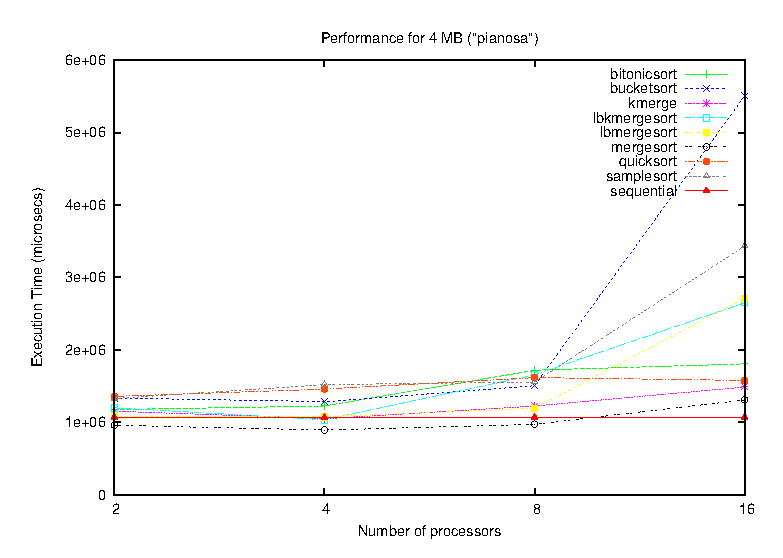
\includegraphics[width=0.4\textwidth]{plots/test_01_pianosa/NxTxA/M1048576_pianosa_NxTxA}} 
	\hspace*{20pt}	
  	\subfloat[Data set of 2M integers.]{\label{NxTxA-2M}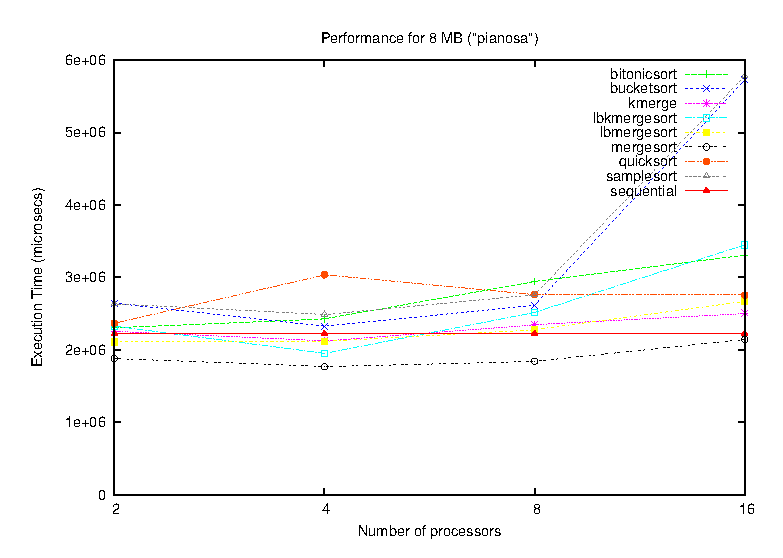
\includegraphics[width=0.4\textwidth]{plots/test_01_pianosa/NxTxA/M2097152_pianosa_NxTxA}} 
  		
	\centering
	\subfloat[Data set of 4M integers.]{\label{NxTxA-4M}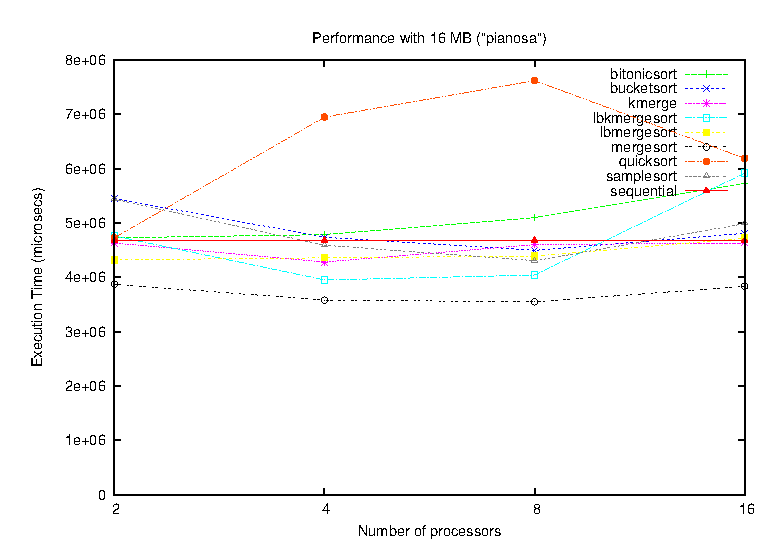
\includegraphics[width=0.4\textwidth]{plots/test_01_pianosa/NxTxA/M4194304_pianosa_NxTxA}} 
  	\hspace*{20pt}
  	\subfloat[Data set of 8M integers.]{\label{NxTxA-8M}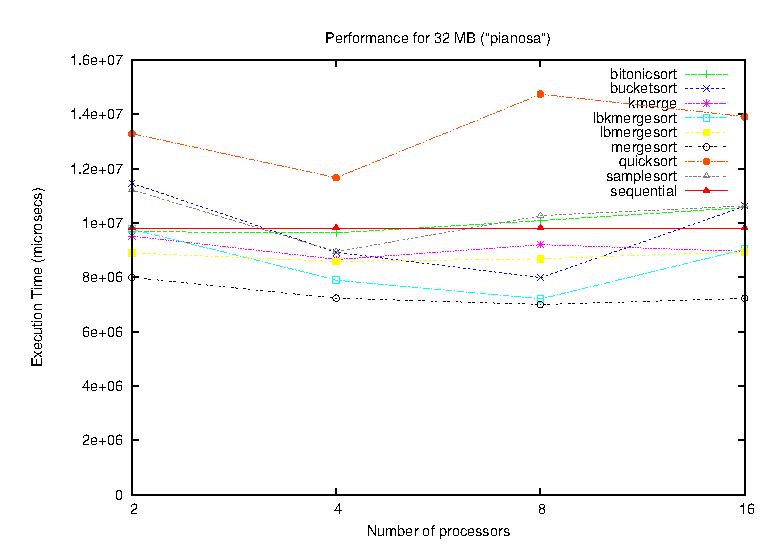
\includegraphics[width=0.4\textwidth]{plots/test_01_pianosa/NxTxA/M8388608_pianosa_NxTxA}} 
	
	\centering
  	\subfloat[Data set of 16M integers.]{\label{NxTxA-16M}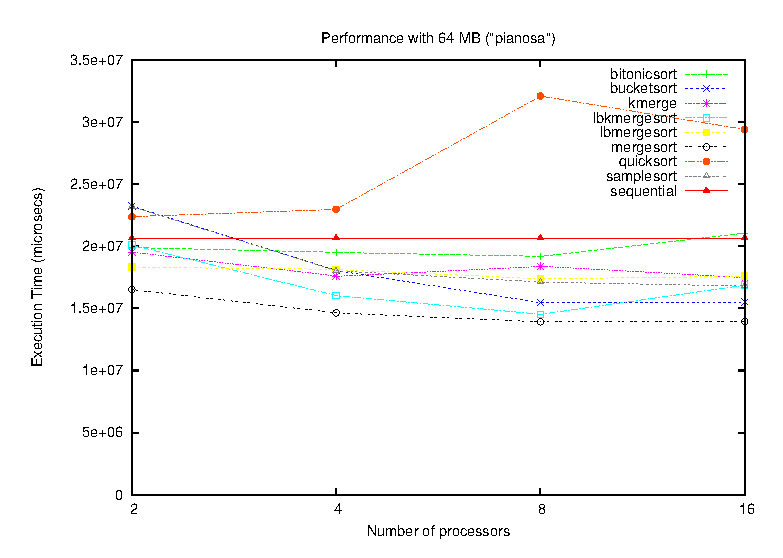
\includegraphics[width=0.4\textwidth]{plots/test_01_pianosa/NxTxA/M16777216_pianosa_NxTxA}}   
  	\hspace*{20pt}  
  	\subfloat[Data set of 32M integers.]{\label{NxTxA-32M}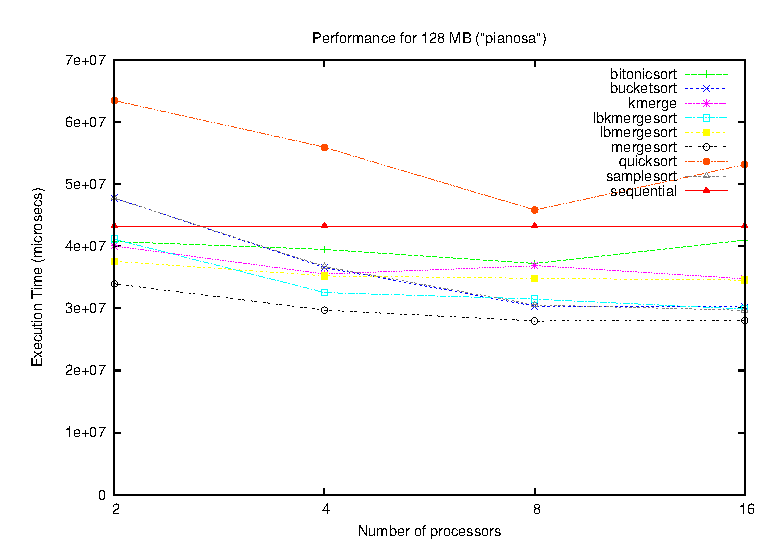
\includegraphics[width=0.4\textwidth]{plots/test_01_pianosa/NxTxA/M33554432_pianosa_NxTxA}} 
  	
	\caption{\textit{Pianosa}. Time Completion for sorting \textit{small} data sets. Each graphic represents a data set of fixed size, while each shape on a graphic shows the Time Completion of a certain Sorting Algorithm for that data set.}
	\label{NxTxA-small}
\end{figure} 

\begin{figure}[!ht]
	\centering
	\subfloat[Data set of 64M integers.]{\label{NxTxA-64M}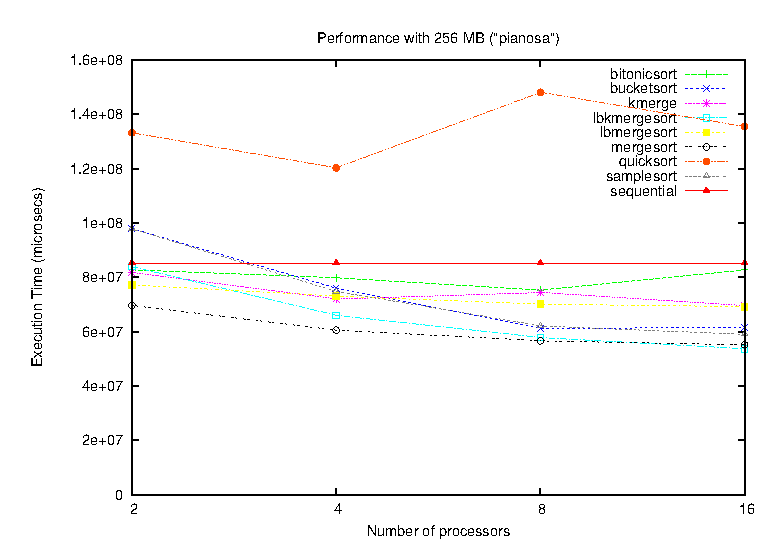
\includegraphics[width=0.5\textwidth]{plots/test_01_pianosa/NxTxA/M67108864_pianosa_NxTxA}} 
	
	\centering
  	\subfloat[Data set of 128M integers.]{\label{NxTxA-128M}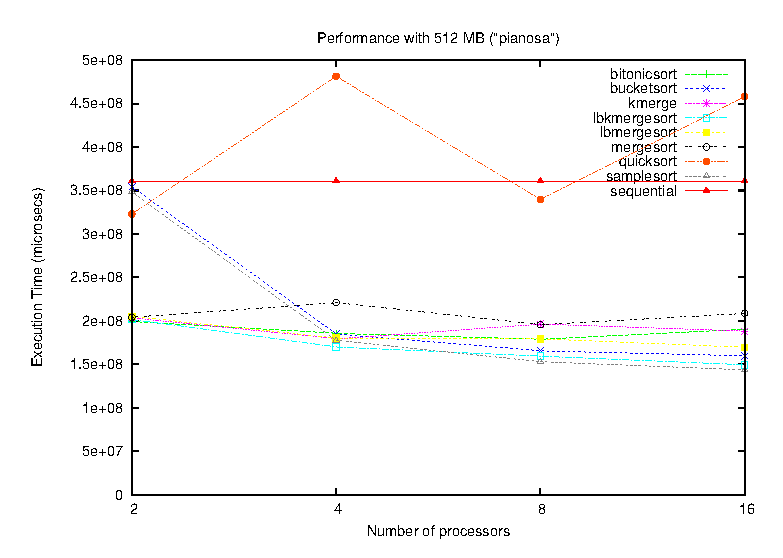
\includegraphics[width=0.5\textwidth]{plots/test_01_pianosa/NxTxA/M134217728_pianosa_NxTxA}} 
  		
	\centering
	\subfloat[Data set of 256M integers.]{\label{NxTxA-256M}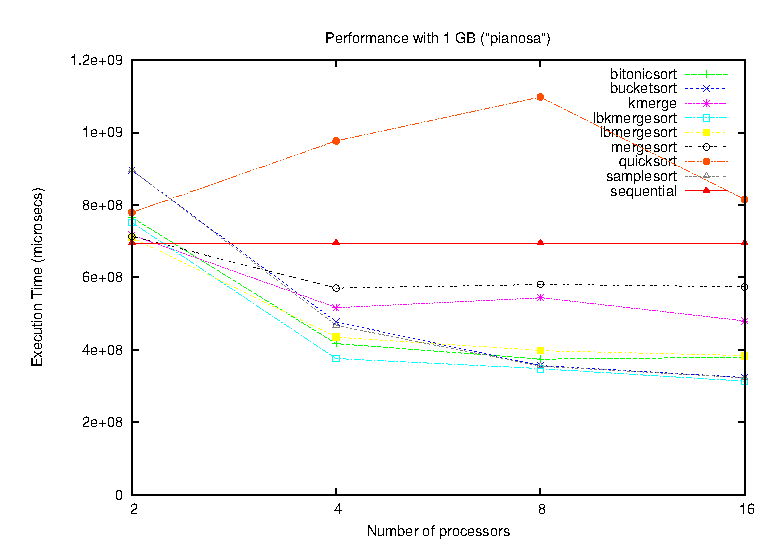
\includegraphics[width=0.5\textwidth]{plots/test_01_pianosa/NxTxA/M268435456_pianosa_NxTxA}} 
  	
  	\caption{\textit{Pianosa}. Time Completion for sorting \textit{large} data sets. Each graphic represents a data set of fixed size, while each shape on a graphic shows the Time Completion of a certain Sorting Algorithm for that data set.}
	\label{NxTxA-large}
\end{figure}

\begin{figure}[!ht]  	
  	\centering
  	\subfloat[Data set of 512M integers.]{\label{NxTxA-512M}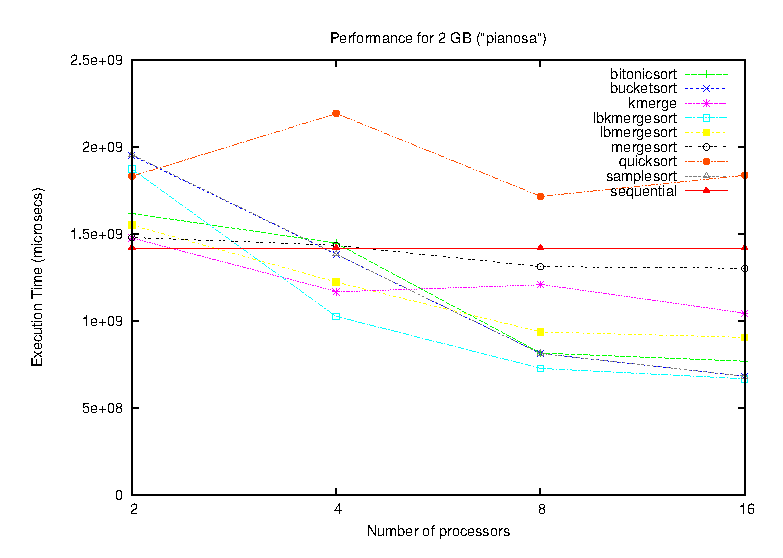
\includegraphics[width=0.6\textwidth]{plots/test_01_pianosa/NxTxA/M536870912_pianosa_NxTxA}} 
	
	\centering
  	\subfloat[Data set of 1G integers.]{\label{NxTxA-1G}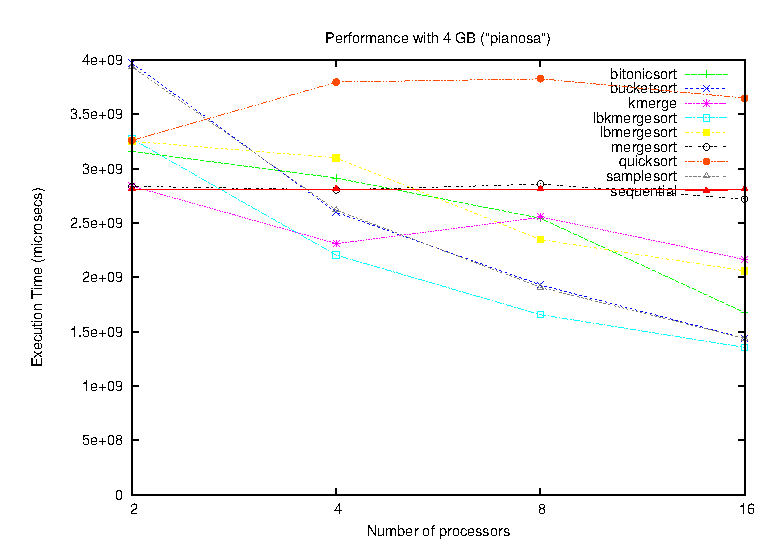
\includegraphics[width=0.6\textwidth]{plots/test_01_pianosa/NxTxA/M1073741824_pianosa_NxTxA}}    
  	
	\caption{\textit{Pianosa}. Time Completion for sorting \textit{huge} data sets. Each graphic represents a data set of fixed size, while each shape on a graphic shows the Time Completion of a certain Sorting Algorithm for that data set.}
	\label{NxTxA-huge}
\end{figure} 

\begin{figure}[!ht]
	\centering
	\subfloat[Parallelism degree 2.]{\label{MxTxA-n2}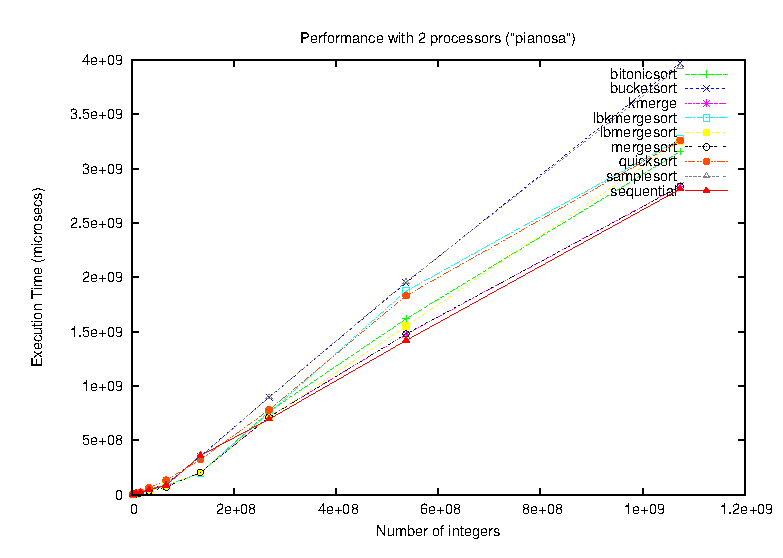
\includegraphics[width=0.4\textwidth]{plots/test_01_pianosa/MxTxA/n2_pianosa_MxTxA}} 
	\hspace*{20pt}	
  	\subfloat[Parallelism degree 4.]{\label{MxTxA-n4}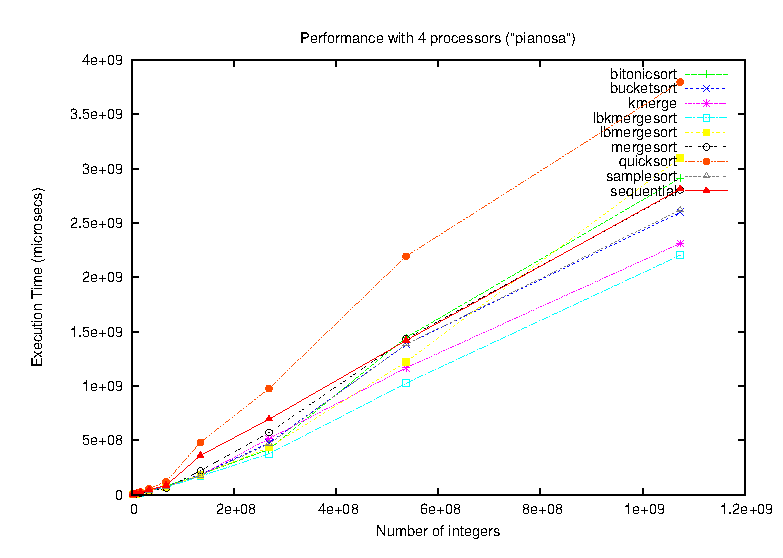
\includegraphics[width=0.4\textwidth]{plots/test_01_pianosa/MxTxA/n4_pianosa_MxTxA}} 
  		
	\centering
	\subfloat[Parallelism degree 8.]{\label{MxTxA-n8}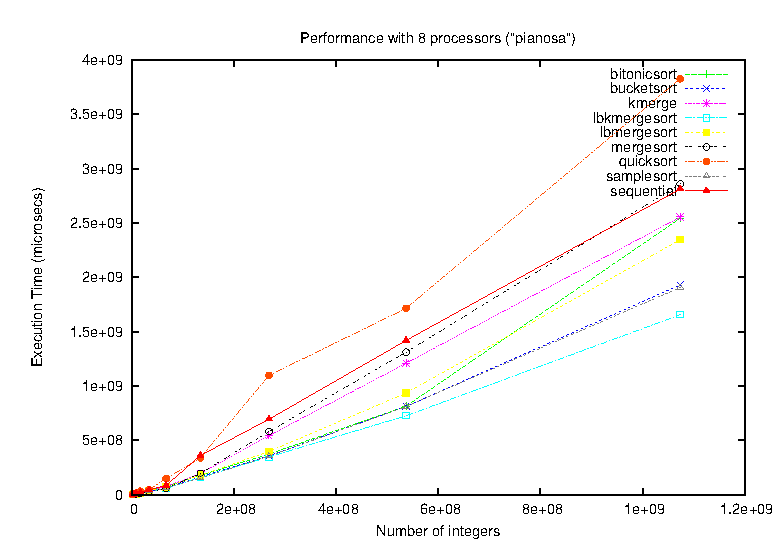
\includegraphics[width=0.4\textwidth]{plots/test_01_pianosa/MxTxA/n8_pianosa_MxTxA}} 
  	\hspace*{20pt}
  	\subfloat[Parallelism degree 16.]{\label{MxTxA-n16}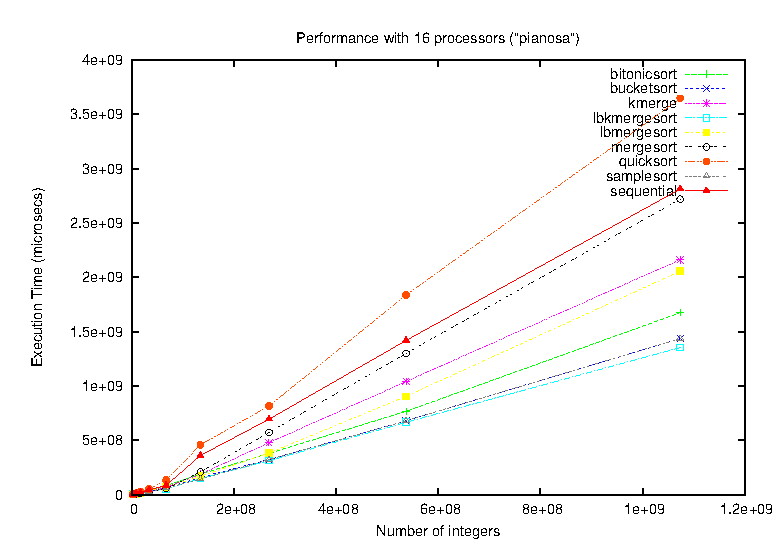
\includegraphics[width=0.4\textwidth]{plots/test_01_pianosa/MxTxA/n16_pianosa_MxTxA}} 
  	
	\caption{\textit{Pianosa}. Time Completion for sorting data sets with fixed parallelism degree.}
	\label{MxTxA}
\end{figure} 

\clearpage
\subsubsection{Intel Xeon X5670}
In this section we analyze the behaviour of Sorting Algorithms on a Chip MultiProcessor (CMP), namely a Symmetric MultiProcessor (SMP) on chip. The CMP in question is the Intel Xeon X5670, described in~\ref{PCM}, which is a generic node of the cluster $PCM$. We will be able to test our algorithms for parallelism degrees up to 8. We expect that performance results on this architecture will be significantly different from the ones obtained on Pianosa, in particular from a \textit{qualitative} point of view. Indeed, there are two key factors: first, the huge amount of primary memory will diminish the overhead due to I/Os; second, the communications now take place in shared memory thus they are less expensive.

\paragraph{Scalability of Sorting Algorithms} Figure~\ref{PCM-NxTxM} and~\ref{PCM-MxTxN} show the time completion of Sorting Algorithms for data sets up to 2 GB. Exactly as on $Pianosa$, due to the fine grain computation, there is not any Sorting Algorithm that shows a good scalability for \textbf{small} data sets. On the other hand, the previous considerations on the primary memory size and the cost of communications justify intuitively why, for \textbf{large} data sets, most Sorting Algorithms scale better than on $Pianosa$ (even if still far away from the ideality). Figure~\ref{PCM-NxTxM} shows that increasing the parallelism degree from 2 to 4, a lot of Sorting Algorithms scale really close to the ideality, while from 4 to 8 there is still a gain, but in general lower. Exactly as on $Pianosa$, \textit{Bucketsort}, \textit{Samplesort} and \textit{Load-Balanced Multi-Way Mergesort} exhibit the best performance in terms of both scalability and time completion. \textit{Mergesort} (Figure~\ref{PCM-NxTxM-mergesort}) was bad on $Pianosa$ because of both the communications overhead and the unbalanced workload, but now exhibit a great scalability up to parallelism degree 8; this is thanks also to the faster hardware which let the last sequential phase of merging becoming less incisive on the overall time completion. Figure~\ref{PCM-NxTxM-quicksort} shows \textit{Quicksort} which has the worst performance TODO. Figure~\ref{PCM-NxTxM-kmerge} shows the bad performance of \textit{4-Way Mergesort}; this algorithm suffers the last phase of merging that, since it is made by a single process (see~\ref{kmerge}), becomes predominant with respect to the gain of the parallelization. 

\begin{figure}[t]
	\begin{center}
		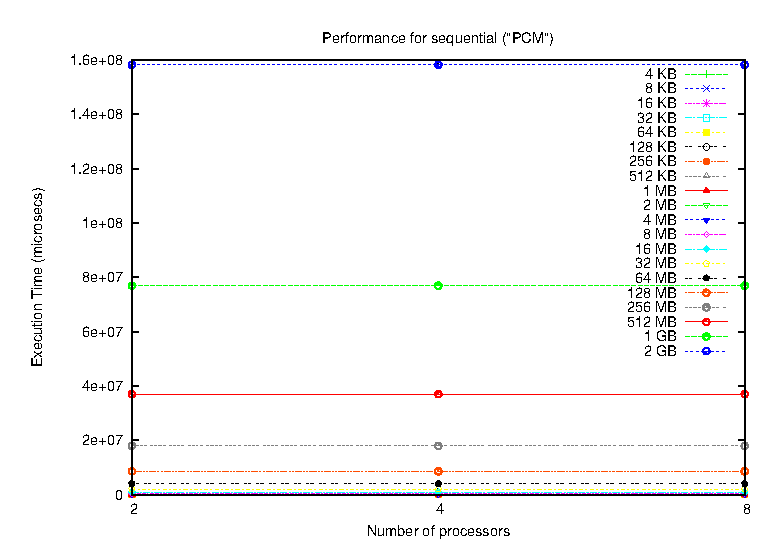
\includegraphics[scale=0.6]{plots/test_00_PCM/NxTxM/sequential_PCM_NxTxM}
	\end{center}
  	\caption{\textit{Intel Xeon X5670}. Completion Time for the Sequentialsort.}
  	\label{sequential-PCM}
\end{figure}

\begin{figure}[h]
	\centering
	\subfloat[Quicksort.]{\label{PCM-NxTxM-sequential}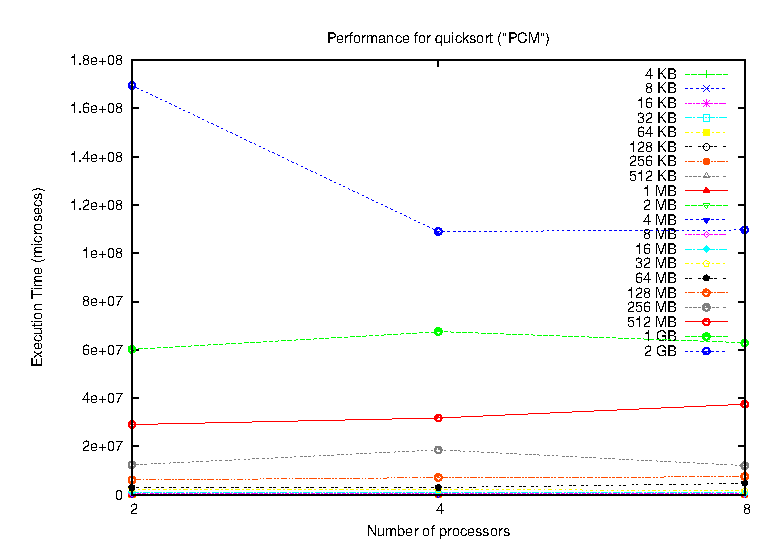
\includegraphics[width=0.4\textwidth]{plots/test_00_PCM/NxTxM/quicksort_PCM_NxTxM}} 
	\hspace*{20pt}	
  	\subfloat[Bitonicsort.]{\label{PCM-NxTxM-bitonicsort}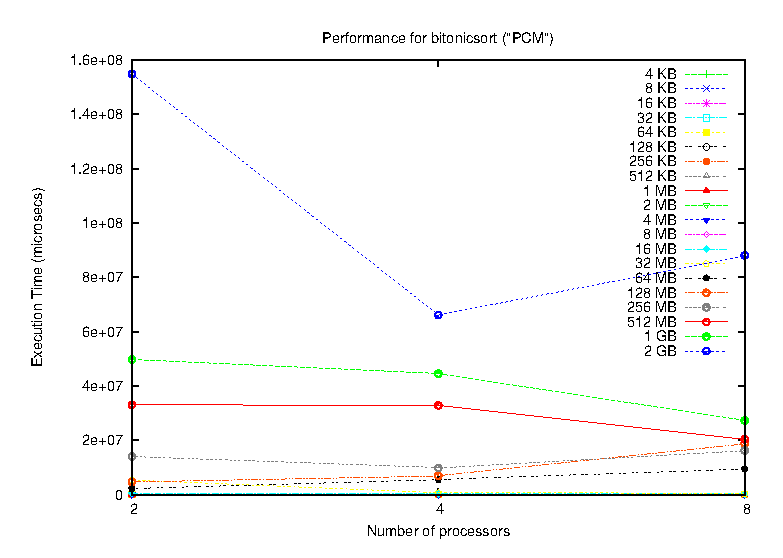
\includegraphics[width=0.4\textwidth]{plots/test_00_PCM/NxTxM/bitonicsort_PCM_NxTxM}} 
	
	\centering
	\subfloat[Bucketsort.]{\label{PCM-NxTxM-bucketsort}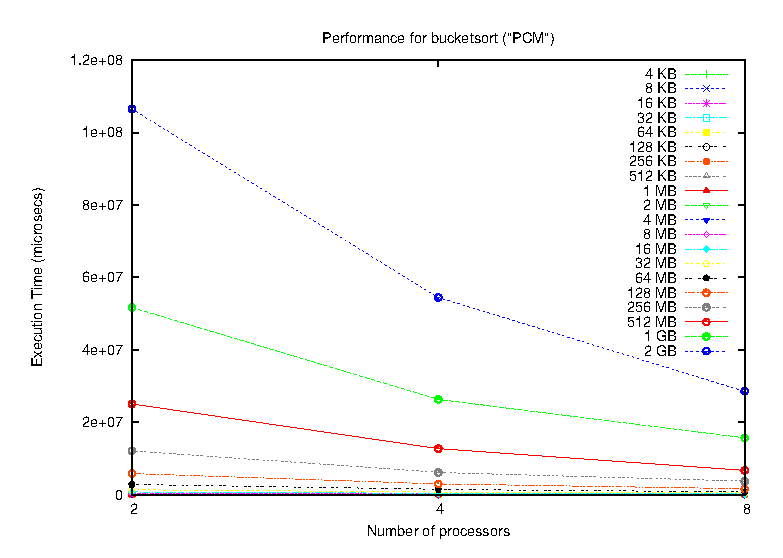
\includegraphics[width=0.4\textwidth]{plots/test_00_PCM/NxTxM/bucketsort_PCM_NxTxM}} 
  	\hspace*{20pt}
  	\subfloat[Samplesort.]{\label{PCM-NxTxM-samplesort}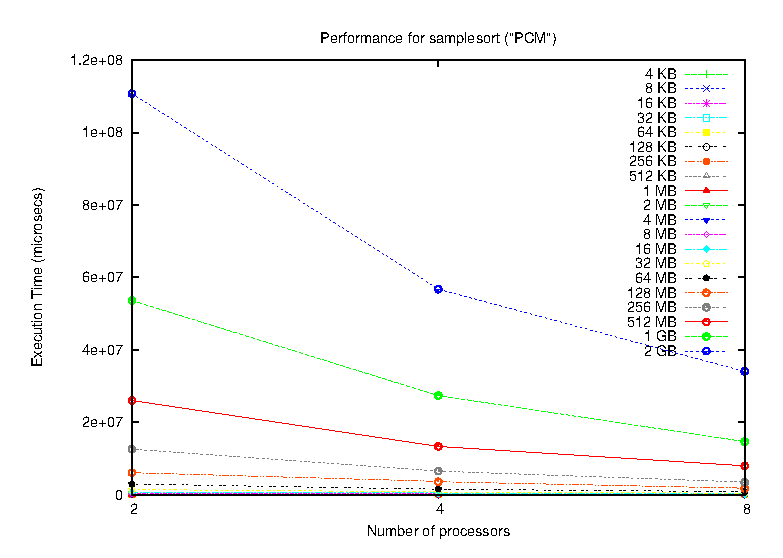
\includegraphics[width=0.4\textwidth]{plots/test_00_PCM/NxTxM/samplesort_PCM_NxTxM}} 
	
	\centering
  	\subfloat[Mergesort.]{\label{PCM-NxTxM-mergesort}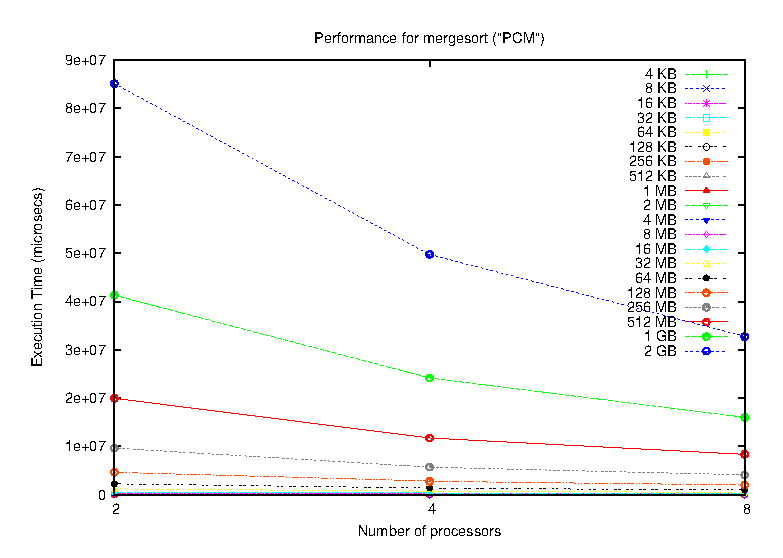
\includegraphics[width=0.4\textwidth]{plots/test_00_PCM/NxTxM/mergesort_PCM_NxTxM}}   
  	\hspace*{20pt}  
  	\subfloat[4-Way Mergesort.]{\label{PCM-NxTxM-kmerge}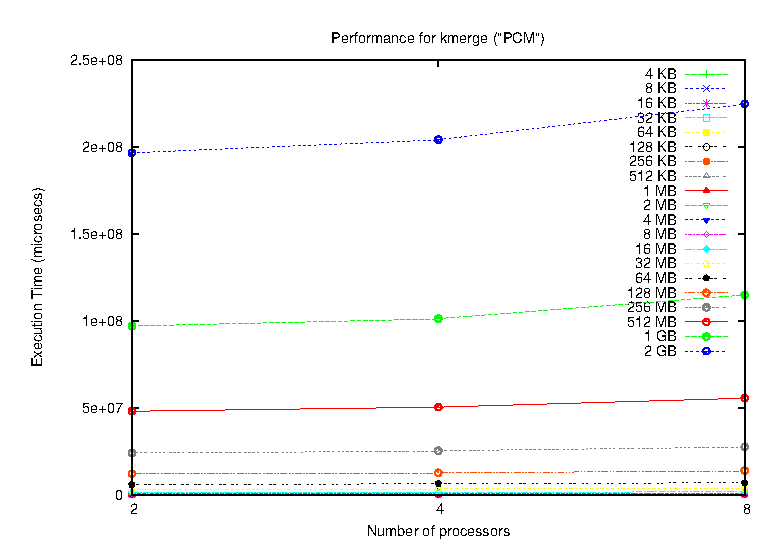
\includegraphics[width=0.4\textwidth]{plots/test_00_PCM/NxTxM/kmerge_PCM_NxTxM}} 
	
	\centering
  	\subfloat[Load-Balanced Mergesort.]{\label{PCM-NxTxM-lbmergesort}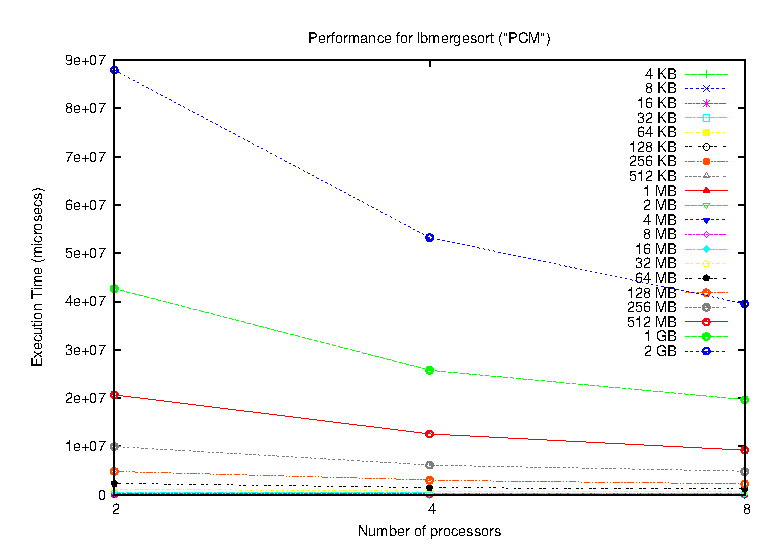
\includegraphics[width=0.4\textwidth]{plots/test_00_PCM/NxTxM/lbmergesort_PCM_NxTxM}} 
  	\hspace*{20pt}  
  	\subfloat[Load-Balanced Multi-Way Mergesort.]{\label{PCM-NxTxM-lbkmergesort}\includegraphics[width=0.4\textwidth]{plots/test_00_PCM/NxTxM/lbkmergesort_PCM_NxTxM}} 	
  	
	\caption{\textit{Intel Xeon X5670}. Time Completion of Sorting Algorithms by varying the parallelism degree. Each shape on a graphic represents the Time Completion of a certain Sorting Algorithm for a data set of specific size.}
	\label{PCM-NxTxM}
\end{figure}
 
\begin{figure}[!ht]
	\centering
	\subfloat[Quicksort.]{\label{PCM-MxTxN-sequential}\includegraphics[width=0.4\textwidth]{plots/test_00_PCM/MxTxN/quicksort_PCM_MxTxN}} 
	\hspace*{20pt}	
  	\subfloat[Bitonicsort.]{\label{PCM-MxTxN-bitonicsort}\includegraphics[width=0.4\textwidth]{plots/test_00_PCM/MxTxN/bitonicsort_PCM_MxTxN}} 
  		
	\centering
	\subfloat[Bucketsort.]{\label{PCM-MxTxN-bucketsort}\includegraphics[width=0.4\textwidth]{plots/test_00_PCM/MxTxN/bucketsort_PCM_MxTxN}} 
  	\hspace*{20pt}
  	\subfloat[Samplesort.]{\label{PCM-MxTxN-samplesort}\includegraphics[width=0.4\textwidth]{plots/test_00_PCM/MxTxN/samplesort_PCM_MxTxN}} 
	
	\centering
  	\subfloat[Mergesort.]{\label{PCM-MxTxN-mergesort}\includegraphics[width=0.4\textwidth]{plots/test_00_PCM/MxTxN/mergesort_PCM_MxTxN}}   
  	\hspace*{20pt}  
  	\subfloat[4-Way Mergesort.]{\label{PCM-MxTxN-kmerge}\includegraphics[width=0.4\textwidth]{plots/test_00_PCM/MxTxN/kmerge_PCM_MxTxN}} 
	
	\centering
  	\subfloat[Load-Balanced Mergesort.]{\label{PCM-MxTxN-lbmergesort}\includegraphics[width=0.4\textwidth]{plots/test_00_PCM/MxTxN/lbmergesort_PCM_MxTxN}} 
  	\hspace*{20pt}  
  	\subfloat[Load-Balanced Multi-Way Mergesort.]{\label{PCM-MxTxN-lbkmergesort}\includegraphics[width=0.4\textwidth]{plots/test_00_PCM/MxTxN/lbkmergesort_PCM_MxTxN}} 
  	
	\caption{\textit{Intel Xeon X5670}. Time Completion of Sorting Algorithms for increasing sizes of the data set. }
	\label{PCM-MxTxN}
\end{figure} 


\paragraph{Comparison between Sorting Algorithms} Figures~\ref{PCM-NxTxA-small} and~\ref{PCM-NxTxA-large} highlight the behaviour of different Sorting Algorithms for specifics sizes of the data set. Notice an interesting aspect reguarding \textbf{small} data sets: we have seen that on $Pianosa$ best algorithms were \textit{qsort} and parallel \textit{Mergesort} (at low parallelism degrees). On this architecture things are deeply different and this is likely due to the fact that processes communications now take place in shared memory. Figure~\ref{PCM-NxTxA-small} shows that most of Sorting Algorithms, altough still far away from the linear scalability, definitely outperform \textit{qsort} (at least for sizes of the data set greater than 8 KB). Moreover, \textit{Mergesort} confirms itself as one of the best Sorting Algorithms both for small data sets and now even for \textbf{large} data sets, together with \textit{Bitonicsort}, \textit{Bucketsort}, \textit{Samplesort} and \textit{Load-Balanced (Multi-Way) Mergesort}.

\begin{figure}[!ht]
	\centering
	\subfloat[Data set of 1K integers.]{\label{PCM-NxTxA-1M}\includegraphics[width=0.4\textwidth]{plots/test_00_PCM/NxTxA/M1024_PCM_NxTxA}} 
	\hspace*{20pt}	
  	\subfloat[Data set of 2K integers.]{\label{PCM-NxTxA-2M}\includegraphics[width=0.4\textwidth]{plots/test_00_PCM/NxTxA/M2048_PCM_NxTxA}} 
  		
	\centering
	\subfloat[Data set of 4K integers.]{\label{PCM-NxTxA-4M}\includegraphics[width=0.4\textwidth]{plots/test_00_PCM/NxTxA/M4096_PCM_NxTxA}} 
  	\hspace*{20pt}
  	\subfloat[Data set of 8K integers.]{\label{PCM-NxTxA-8M}\includegraphics[width=0.4\textwidth]{plots/test_00_PCM/NxTxA/M8192_PCM_NxTxA}} 
	
	\centering
  	\subfloat[Data set of 16K integers.]{\label{PCM-NxTxA-16M}\includegraphics[width=0.4\textwidth]{plots/test_00_PCM/NxTxA/M16384_PCM_NxTxA}}   
  	\hspace*{20pt}  
  	\subfloat[Data set of 32K integers.]{\label{PCM-NxTxA-32M}\includegraphics[width=0.4\textwidth]{plots/test_00_PCM/NxTxA/M32768_PCM_NxTxA}} 
  	
	\centering
  	\subfloat[Data set of 64K integers.]{\label{PCM-NxTxA-16M}\includegraphics[width=0.4\textwidth]{plots/test_00_PCM/NxTxA/M65536_PCM_NxTxA}}   
  	\hspace*{20pt}  
  	\subfloat[Data set of 128K integers.]{\label{PCM-NxTxA-32M}\includegraphics[width=0.4\textwidth]{plots/test_00_PCM/NxTxA/M131072_PCM_NxTxA}}   	
  	
	%\caption{\textit{Intel Xeon X5670}. Time Completion for sorting \textit{small} data sets. Each graphic represents a data set of fixed size, while each shape on a graphic shows the Time Completion of a certain Sorting Algorithm for that data set.}
	%\label{PCM-NxTxA-small}
\end{figure} 

\begin{figure}[!ht]
	\ContinuedFloat
	\centering
	\subfloat[Data set of 256K integers.]{\label{PCM-NxTxA-1M}\includegraphics[width=0.4\textwidth]{plots/test_00_PCM/NxTxA/M262144_PCM_NxTxA}} 
	\hspace*{20pt}	
  	\subfloat[Data set of 512K integers.]{\label{PCM-NxTxA-2M}\includegraphics[width=0.4\textwidth]{plots/test_00_PCM/NxTxA/M524288_PCM_NxTxA}} 

	\centering
	\subfloat[Data set of 1M integers.]{\label{PCM-NxTxA-1M}\includegraphics[width=0.4\textwidth]{plots/test_00_PCM/NxTxA/M1048576_PCM_NxTxA}} 
	\hspace*{20pt}	
  	\subfloat[Data set of 2M integers.]{\label{PCM-NxTxA-2M}\includegraphics[width=0.4\textwidth]{plots/test_00_PCM/NxTxA/M2097152_PCM_NxTxA}} 
  		
	\centering
	\subfloat[Data set of 4M integers.]{\label{PCM-NxTxA-4M}\includegraphics[width=0.4\textwidth]{plots/test_00_PCM/NxTxA/M4194304_PCM_NxTxA}} 
  	\hspace*{20pt}
  	\subfloat[Data set of 8M integers.]{\label{PCM-NxTxA-8M}\includegraphics[width=0.4\textwidth]{plots/test_00_PCM/NxTxA/M8388608_PCM_NxTxA}} 
	
	\centering
  	\subfloat[Data set of 16M integers.]{\label{PCM-NxTxA-16M}\includegraphics[width=0.4\textwidth]{plots/test_00_PCM/NxTxA/M16777216_PCM_NxTxA}}   
  	\hspace*{20pt}  
  	\subfloat[Data set of 32M integers.]{\label{PCM-NxTxA-32M}\includegraphics[width=0.4\textwidth]{plots/test_00_PCM/NxTxA/M33554432_PCM_NxTxA}} 
  	
	\caption{\textit{Intel Xeon X5670}. Time Completion for sorting \textit{small} data sets. Each graphic represents a data set of fixed size, while each shape on a graphic shows the Time Completion of a certain Sorting Algorithm for that data set.}
	\label{PCM-NxTxA-small}
\end{figure} 

\begin{figure}[!ht]
	\centering
	\subfloat[Data set of 64M integers.]{\label{PCM-NxTxA-64M}\includegraphics[width=0.4\textwidth]{plots/test_00_PCM/NxTxA/M67108864_PCM_NxTxA}} 
	\hspace*{20pt}	
  	\subfloat[Data set of 128M integers.]{\label{PCM-NxTxA-128M}\includegraphics[width=0.4\textwidth]{plots/test_00_PCM/NxTxA/M134217728_PCM_NxTxA}} 
  		
	\centering
	\subfloat[Data set of 256M integers.]{\label{PCM-NxTxA-256M}\includegraphics[width=0.4\textwidth]{plots/test_00_PCM/NxTxA/M268435456_PCM_NxTxA}} 
  	\hspace*{20pt}
  	\subfloat[Data set of 512M integers.]{\label{PCM-NxTxA-512M}\includegraphics[width=0.4\textwidth]{plots/test_00_PCM/NxTxA/M536870912_PCM_NxTxA}} 
	
	\caption{\textit{Intel Xeon X5670}. Time Completion for sorting \textit{large} data sets. Each graphic represents a data set of fixed size, while each shape on a graphic shows the Time Completion of a certain Sorting Algorithm for that data set.}
	\label{PCM-NxTxA-large}
\end{figure} 

\begin{figure}[!ht]
	\centering
	\subfloat[Parallelism degree 2.]{\label{PCM-MxTxA-n2}\includegraphics[width=0.5\textwidth]{plots/test_00_PCM/MxTxA/n2_PCM_MxTxA}} 
	
	\centering
  	\subfloat[Parallelism degree 4.]{\label{PCM-MxTxA-n4}\includegraphics[width=0.5\textwidth]{plots/test_00_PCM/MxTxA/n4_PCM_MxTxA}} 
  		
	\centering
	\subfloat[Parallelism degree 8.]{\label{PCM-MxTxA-n8}\includegraphics[width=0.5\textwidth]{plots/test_00_PCM/MxTxA/n8_PCM_MxTxA}} 
  	
	\caption{\textit{Intel Xeon X5670}. Time Completion for sorting data sets with fixed parallelism degree.}
	\label{PCM-MxTxA}
\end{figure}

\clearpage

\subsubsection{PCM}
$PCM$ is a cluster of shared memory machines, thus all considerations reguarding mapping of processes to cores made in~\ref{fram-intr} become matter of study. Even the official guide of \textit{mvapich2}, the version of MPI that we have used to exploit Infiniband, emphasizes the importance of process-to-core mapping: as shown in~\cite{MVAPICH2-MAPPING}, different allocations of processes to cores can have a significant impact on the cost of communications. In principle, an entire study could be dedicated to this topic, leading to a lot of possible mappings, each one based on its reasonable heuristic. Obviously, we had to limit our analysis to a subset of the most simple mappings. In particular, we have studied the following configurations:   
\begin{itemize}
\item \textbf{Sequential mapping}. Adjacent ranks mapped on adjacent \textit{cores}. E.g., given two CPUs each one with 4 cores and 8 MPI processes, rank 0 goes on the first core of the \textit{first} CPU, rank 1 goes on the second core of the \textit{first} CPU, ..., rank 5 goes on the first core of the \textit{second} CPU and so on.
\item \textbf{Interleaved mapping}. Adjacent ranks mapped on adjacent \textit{CPUs}. E.g., given two CPUs each one with 4 cores and 8 MPI processes, rank 0 goes on the first core of the \textit{first} CPU, rank 1 goes on the first core of the \textit{second} CPU, rank 2 goes on the second core of the \textit{first} CPU and so on.
\item \textbf{Algorithm-specific mapping}. We have also studied a few mapping based on the nature of a specific Sorting Algorithm, like \textit{Mergesort} and \textit{Quicksort}. For instance, a mapping could be designed to let the most critical part of a stencil to take place in shared memory rather than inter-node.  
\end{itemize}
In the following, we will consider only the \textit{sequential mapping} because we have practically experienced that collective communications (in particular, the \textit{gather}) are more cost-effective than for other mappings. For more informations about the results obtained with other mappings the reader could refer to specific material attached to this report.


\paragraph{Scalability of Sorting Algorithms}

\paragraph{Comparison between Sorting Algorithms}

\clearpage


\subsection{Comparing the results}